\section{Details on Estimation, Interpolation, and Extrapolation} \label{appendix:methodology}

\noindent We provide details on the approach to estimate treatment effects out of sample. The difference in the approach for each outcome is based on different scenarios of data availability.

\subsection{Complete Data}
\label{app:method_fullobs}

\noindent  In the case where we have complete data, we only need to address compromised randomization. Appendix~\ref{appendix:assessingcc} shows that our estimates are not sensitive to alternative approaches to compromised randomization. Our baseline estimates throughout this paper do not account for this. By complete data, we mean that we observe the data for at least 90\% of the individuals in the sample. Table~\ref{table:nonipw} lists the variables that are completely observed.\\

\noindent For these outcomes, we estimate the standard errors of our estimates by resampling the ABC/CARE data. We estimate non-parametric $p$-values based on the bootstrap distribution. We perform inference in this same way throughout the paper.

\begin{table}[H]
\begin{threeparttable}
\caption{Variables Estimated without IPW Adjustment}
\label{table:nonipw}
\centering
% CONTENT CREATED ON SPREADSHEET, TREAT AS A .CSV (TAB DELIMITED)
% CAN BE COPIED INTO A SPREADSHEET PROGRAM (EXCEL, LIBRECALC) FOR EDITING
\begin{tabular}{l l}
\toprule
Variable	&	Age	\\
\midrule			
IQ Standard Score	&	2, 3, 4, 5, 6, 7, 8, 12, 15, 21	\\
PIAT Math Standard Score	&	7	\\
Home Total Score	&	0.5, 1.5, 2.5, 3.5, 4.5, 8	\\
Mother Works	&	2, 3, 4, 5	\\
Biological Mother's Education Level	&	2, 3, 4, 5, 9	\\
Father is Home	&	2, 3, 4, 5	\\
Ever Adopted	&		NA \\
Graduated High School	&	NA	\\
Attended Vocation/Tech/Community College	&	NA	\\
Earned Degree from 4-year College	&	NA	\\
Years of Education	&	30	\\
Works a Job	&	30	\\
Total Felony Arrests	&	Mid-30s	\\
Total Misdemeanor Arrests	&	Mid-30s	\\
Total Years Incarcerated	&	30	\\
Self-reported Health	&	30	\\
Number of Cigarettes Smoked Per Day Last Month	&	30	\\
Number of Days Drank Alcohol Last Month	&	30	\\
Number of Days Binge Drank Alcohol Last Month	&	30	\\
Program Costs	&	0--26	\\
Control Contamination Costs	&	0--26	\\
Education Costs	&	0--26	\\
Medical Expenditure &	8--30	\\
Justice System Costs	&	0--50	\\
Prison Costs	&	0--50	\\
Victimization Costs	&	0--50	\\
\bottomrule			
\end{tabular}
\begin{tablenotes}
\footnotesize
\item Note: The table above lists the variables for which we do not apply IPW when estimating
treatment effects.
\end{tablenotes}
\end{threeparttable}
\end{table}

\subsection{Partially Complete Data}
\label{app:method_partialobs}

\noindent When we do not observe data on an outcome for more than 10\% of the individuals in the sample, we consider the outcome to be partially complete. These outcomes include: parental income at ages 2, 3, 4, 5, 9, 12, and 15, for which we observe no more than 91 subjects at any given age; and the health survey at age 34, for which we observe no more than 72 subjects.\\

\noindent For partially complete outcomes, we correct for attrition using an inverse probability scheme (IPW) as in  \citet{Horvitz_Thompson_1952_JASA}. To estimate the propensity to respond, we estimate a logit model of observing the outcome,
controlling for treatment status and three additional covariates. The additional covariates are
chosen among a set of variables, as detailed in Appendix~\ref{appendix:bvariables}. See Appendix~\ref{appendix:attrition} for a derivation of the (IPW) scheme and for a list of the variables we use to construct it for each partially complete variables. Whenever we use IPW, we account for the sampling variation implied in the estimation by the scheme when producing our bootstrap-based inference.\\

\noindent In each of the estimates we present in this paper, we allow the reader to assess the sensibility that the estimates have to accounting for IPW. In Table~\ref{table:tescombined}, where we present our main estimates, we present estimates for the first counterfactual of our interest (``Treatment vs. Next Best'') without accounting for IPW in column (1). In column (2), we present estimates accounting for IPW. The rest of the columns display similar exercises for the other counterfactuals we consider. For the rest of the outcomes that do not appear in Table~\ref{table:tescombined}, we present this same information in Appendix~\ref{appendix:results}.\footnote{We only account for IPW for the list of variables listed here, or any calculation involving them.}

\subsection{Incomplete Data}
\label{app:method_noobs}

\noindent We do not observe life-cycle profiles for outcomes that are crucial for estimating the life-cycle benefits of ABC/CARE. The main examples are parental income, subject labor income, public-transfer income, and health-related variables. The importance of the first one is that ABC/CARE, in practice, had a childcare feature. It relaxed the time constraints of the mothers of the treated children, who therefore were able to study or to work more. Potentially, this shifted the life-cycle profile of the mothers, either by allowing them to have more schooling or more work experience. We estimate these profiles. Similarly, a comprehensive evaluation accounts for the effect on the whole life-cycle profile of subject labor income and public-transfer income. We follow the strategy in Section~\ref{section:cbamethodology} to identify and estimate these profiles, i.e. to produce predictions.

\subsubsection{Subject and Transfer Income}

\noindent Labor income and public-transfer income of subjects are only observed at ages 21 and 30.\footnote{At age 21, public-transfer income includes Aid to Families with Dependent Children (AFDC) subsidies, food stamps, survivor benefits, disability benefits, social security, rent subsidies, and fuel subsidies. At age 30, public-transfer income includes food stamps, welfare, housing assistance, workman's compensation, disability, social security, supplemental security income, unemployment benefits, worker's compensation insurance, fuel subsidies, educational and aid grants, and other forms of welfare.} For all other ages, we produce a prediction (either an interpolation or an extrapolation). We explain and justify the variables we use to predict below.

\subsubsection{Parental Income}

\noindent We devote a self-contained section for parental income because we use a different procedure. We justify this decision and explain the data sources in Appendix~\ref{app:parentalincome}.

\subsection{Auxiliary Datasets and Variables Used to Predict}

\subsubsection{Auxiliary Datasets}

\noindent We rely on the following datasets to estimate life-cycle profiles. We use this data in a very similar fashion to estimate the three life-cycle profiles of interest. For subject's labor income and parental labor income we use the exact same data. Two differences are: (i) for parental income, we need to produce a life-cycle profile from where the child is zero years old to when her mother is 65 (age at which we assume she retires); (ii) for parental income, we observe more years, and therefore need to produce predictions for fewer time points. A brief description of the auxiliary or non-experimental datasets and their use follows.\\

\noindent \textbf{The National Longitudinal Survey of Youth (NLSY79)} is a longitudinal survey beginning in 1979 that follows individuals born between 1957 and 1964. The initial interview included 12,686 respondents aged 14 to 22. The survey was designed to include 6,111 individuals representing the non-institutionalized civilian population, a supplemental sample of 5,295 civilian Hispanics, Latinos, blacks, non-blacks/non-Hispanics, and economically disadvantaged youth, and a sample of 1,280 who served in the military as of September 30, 1978. When appropriately weighted, the NLSY79 is nationally representative of the youth living in the U.S. on January 1, 1979. We include individuals from all three subsamples in our analysis. \\

\noindent The NLSY79 collected data on labor market participation, education, family background, family life, health issues, assets and income, government program participation, and measures of cognitive skills. We use these data for our estimation from ages 31 to 67.\\

\noindent We restrict the NLSY79 sample to individuals with labor income less than \$300,000 (2014 USD) at any given year. We \textit{do not} do this to match the individuals in the NLSY79 to the individuals in ABC/CARE. Instead, we do it to avoid estimating our predictions with outliers in the auxiliary sample.\footnote{For details on how we match the individuals in the experimental sample to the individuals in the non-experimental sample, see Appendix~\ref{appendix:match}}. With the mean labor income (2014 USD) in the ABC/CARE sample being \$32,782 at age 30, and the maximum reported being \$189,938, the cut-off we impose on the auxiliary data is high enough so that the labor income support at age 30 in ABC/CARE is contained in the support of labor income at age 30 in the NLSY79.\footnote{For labor income at age 21, we use the CNLSY.}\\

\noindent We do not impose a restriction on birth year on the NLSY79 as all respondents are age between 47 and 55 at the time of the last interview (conducted in 2012). This age range is within the 31--67 range for which we extrapolate the income of the ABC/CARE subjects. \\

\noindent Given the biennial nature of the NLSY79, we only observe each subject at either odd or even ages. Not only does this reduce the size of the sample on which we fit our prediction model at each age, but it can introduce biases associated with the odd-aged and even-aged cohorts. To address this issue, we perform a linear interpolation on the variables in the NLSY79 data that enter into our prediction model. This allows us to estimate our prediction model on all subjects of the NLSY79 satisfying our restrictions at every age. \\

\noindent \textbf{The Children of the National Longitudinal Survey of Youth (CNLSY)} is a survey of the children of the mothers from the NLSY79, beginning in 1986. At the time of the initial interview, the ages of the children surveyed ranged from 0 to 23. As of 2010, the CNLSY sample includes 11,504 children born to NLSY79 mothers. With appropriate weights, the CNLSY may be considered nationally representative of children born to women who were aged 14 to 22 during 1979. Interviews were conducted annually between 1986 and 1994, and biennially thereafter. \\

\noindent Similar to the NLSY79, the CNLSY collected data on cognitive ability, motor and social development, home environment, health information, education, attitudes, employment, income, family decisions, and more. We use these data to estimate a prediction model for subject income for ages 22 through 29. \\

\noindent As we did with the NLSY79 and for the same reasons, we restrict the CNLSY sample to individuals with labor income less than \$300,000 (2014 USD) at any given year. In addition to this, we limit the sample to subjects born between 1978 and 1983. Because the CNLSY data extends to 2012, this implies that we use the most recent data from the CNLSY in which individuals are aged 29 to 34. Finally, given the biennial nature of the survey, we perform a linear interpolation on the variables that enter into our prediction model. This allows us to use as much of the CNLSY data as possible at every age when interpolating subject income. \\

\noindent \textbf{The Panel Survey of Income Dynamics (PSID)} is a longitudinal household survey containing between 5,000 and 8,500 families in each wave. It began as a yearly survey in 1968 and has been fielded biennially since 1996. When appropriately weighted, the PSID is designed to be representative of U.S. households. The PSID provides extensive information concerning demographics, economic outcomes, health outcomes, marriage and fertility, and more. In addition to using the PSID to predict future earnings of ABC/CARE subjects, we use the PSID to predict health outcomes. See Appendix \ref{section:data_psid} for details on how the PSID relates to health outcomes. \\

\noindent Similar to the CNLSY, we restrict the PSID to individuals born between 1945 and 1981. Because the data extend to 2013, we use the most recent subsample of individuals aged 30 to 67. We also exclude all individuals with labor income exceeding \$300,000 (2014 USD) in any given year for the same reasons. Finally, given the biennial nature of the survey, we perform a linear interpolation on the variables that enter into our prediction model. This allows us to use as much of the PSID data as possible at every age to interpolate subject income. \\

\subsubsection{Variables Used to Predict}

\noindent We base our predictions of a generic outcome, $Y_{t}$ on background (pre-treatment) variables, $\bm{B}$, and variables that could have been affected by treatment $\bm{X}_{t}$. $\bm{X}_{t}$ can contain lagged values (or predictions) of $Y_{t}$.\\

\noindent Our prediction is based on identifying and estimating a relationship between the outcome we want to predict at time $t$, $Y_{t}$, in the non-experimental samples and then using the fitted relationship in the experimental samples. We produce one prediction for each outcome at each point of time. \\

\noindent To be considered a prediction variable, the variable must satisfy three conditions: (i) it has to be available in the experimental and non-experimental samples; (ii) it has to have predictive power on the predicted outcome. Any test of predictive power is arbitrary, because it requires a predictive variable to satisfy certain correlation condition with the predicted outcome. In our case, all the coefficients of a regression of the predicted variable on \textit{all} the prediction variables are chosen to be statistically significant at the 1\% level. We interpret that as evidence of predictive power on the outcome; (iii) the support of the non-experimental samples contains the support of the experimental sample, as we formalize in  Section~\ref{section:methodology},  Assumption~\ref{ass:contain}.\\

\noindent For a variable to satisfy restrictions (i) and (ii), it needs to be the case not only that the variable is available in the non-experimental sample but also that the survey question for it was introduced far enough back in time for us to observe it in a range that is common to the range in which we observe the variables in the experimental sample. To illustrate this, consider the case of body-mass index in the PSID. Survey questions for this variable were introduced in the late 1990s. The sample for which the question was introduced, however, does not span enough observations for its support to cover the support of the experimental sample.\\

\noindent An alternative we follow to lower this problem is to pool diverse auxiliary datasets to maximize the amount of prediction variables we are able to use. As we explain before, we use different non-experimental sources (and therefore different variables) produce our predictions at different ages.\\

\noindent For the two outcomes we predict using this methodology (parental income, subject labor income, and transfer income), the prediction variables we use are: male and a black indicator ($\bm{B}$) in NLSY79, CNLSY, and PSID; mother's education in CNLSY ($\bm{B}$); PIAT scores at ages 5-7 \footnote{We take the average of the PIAT across ages 5 to 7. For ABC, we observe this variable. For CARE, we use the mathematics section of the Woodcock Johnson at these same ages because we do not observe PIAT.} in CNLSY ($\bm{X}_{t}$); years of education at age 30 and labor income at ages 21 and 30 in NLSY79, CNLSY, and PSID ($\bm{X}_{t}$). In CNLSY, we also use the body-mass index at age 34. All these variables are available in the experimental sample. In addition, we use the lagged variable of the predicted variables as a prediction variable (which in most cases is itself predicted).\footnote{At age 21, we start the predictions for subject labor income. We do no predict because we observe those values in the ABC/CARE data. At age 22, we predict using the lagged variable (which we observe). At age 23, we use the prediction at age 22 as a predictor. These illustrates how we predict based on the lagged (observed) variable or on its prediction.} \\

\noindent We use CNLSY to predict between ages 21 and 30 and pool NLSY79 and PSID to predict from age 30 to retirement (age 65, by assumption). We provide tests for restrictions (i) and (ii) next and then discuss potential sensitivity to the choice of these variables.

\subsubsection{Matching the Experimental and Non-experimental Samples} \label{appendix:match}

\noindent When producing our predictions, we have two alternatives: (i) directly use the auxiliary samples; or (ii) use a weighted version of the auxiliary samples so that they more closely align with respect to observed characteristics. We follow the second alternative and match the experimental and auxiliary or non-experimental samples following the procedure in Section~\ref{sec:necrosis}. We construct the weights using the Mahalanobis metric of equation \eqref{eq:ingrownnail} of Section~\ref{sec:necrosis}. This allows us to weigh the individuals in the non-experimental samples to match them on observed characteristics to the individuals using the Mahalanobis metric based on male and black indicators, year of birth, years of education at age 30, and labor income at age 30. We choose these variables because they are available in all three non-experimental samples and we intend to locate common comparison samples.

\paragraph{Sensitivity Analysis to Variables Used to Match}

\noindent To study the sensitivity of our predictions to the choice of different matching variables, we predict income using the following different sets of variables: (i) the baseline matching variables (male and black indicators, year of birth, years of education at age 30, and labor income at age 30); (ii) pre-treatment variables only (male and black indicators and year of birth); and (iii) post-treatment variables (years of education at age 30 and labor income at age 30). Figure~\ref{fig:matchvariables} displays the results of this exercise. The top row represents the exercise for females and the bottom row for males. The predictions exhibit little sensitivity to the choice of matching variables within the set that we experiment with.

\textbf{[JJH: Can we report $R^2$ among the different procedures?] [JLG: Yes. you can see this in Tables C2-C5. There are no interesting changes across ages, but we can plot $R^2$ as a function of age of prediction. I doubt is very insightful.] }

\begin{sidewaysfigure}[H]
\centering
\caption{Predicted Labor Income Profiles, Varying the Matching Variables}\label{fig:matchvariables}
\begin{subfigure}[h]{0.3\textwidth}
		\centering
		\caption{Pre-treatment Variables, Females}
		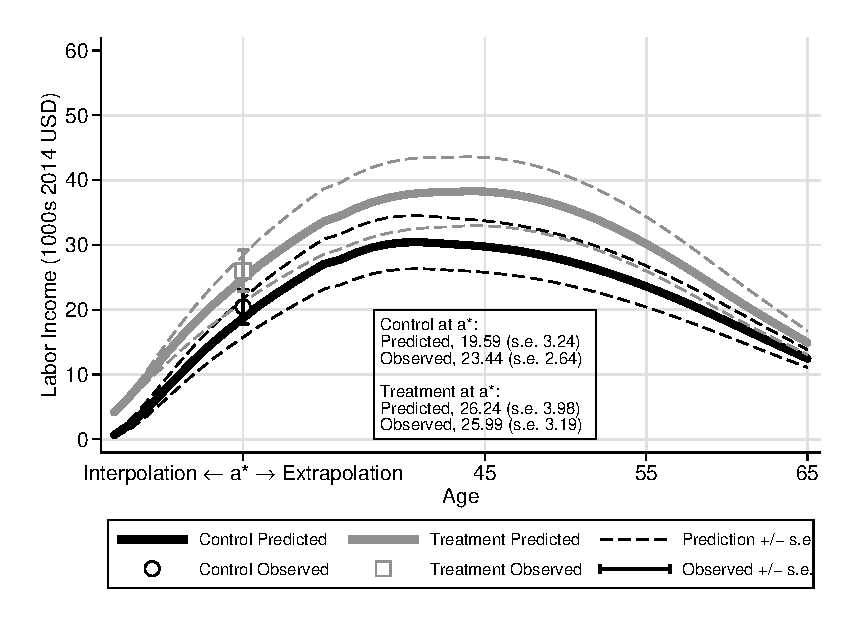
\includegraphics[width=\textwidth]{output/labor_25-65_pset1_mset1_female.eps}
\end{subfigure}%
\begin{subfigure}[h]{0.3\textwidth}
	\centering
	\caption{Post-treatment Variables, Females}
		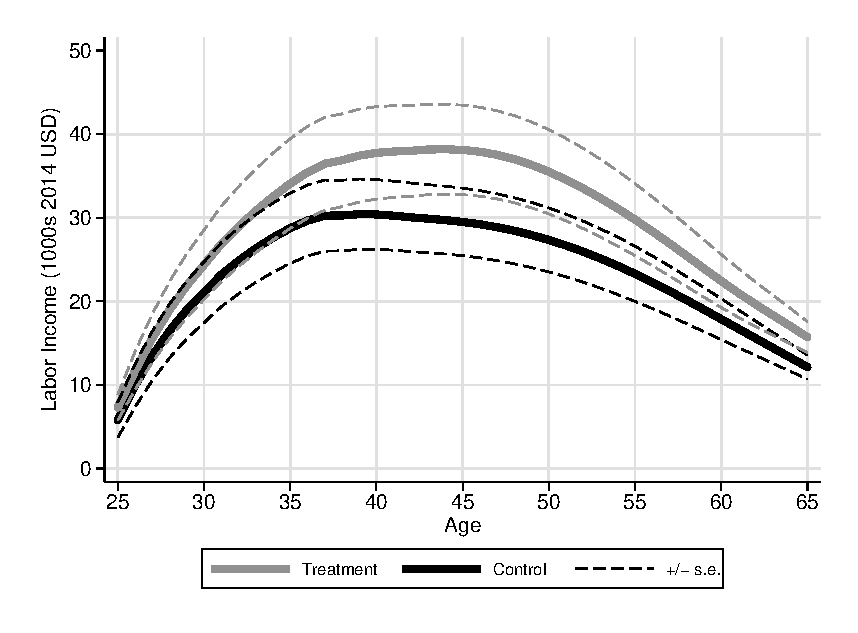
\includegraphics[width=\textwidth]{output/labor_25-65_pset1_mset2_female.eps}
\end{subfigure}%
\begin{subfigure}[h]{0.3\textwidth}
	\centering
	\caption{Pre- and Post-treatment Variables, Females}
		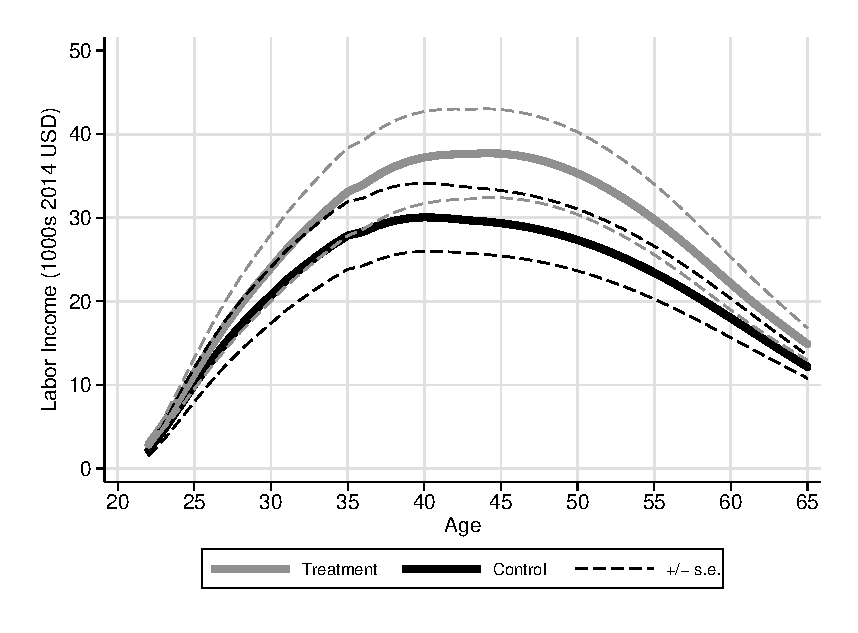
\includegraphics[width=\textwidth]{output/labor_25-65_pset1_mset3_female_sensitivity.eps}
\end{subfigure}
\begin{subfigure}[h]{0.3\textwidth}
		\centering
		\caption{Pre-treatment Variables, Males}
		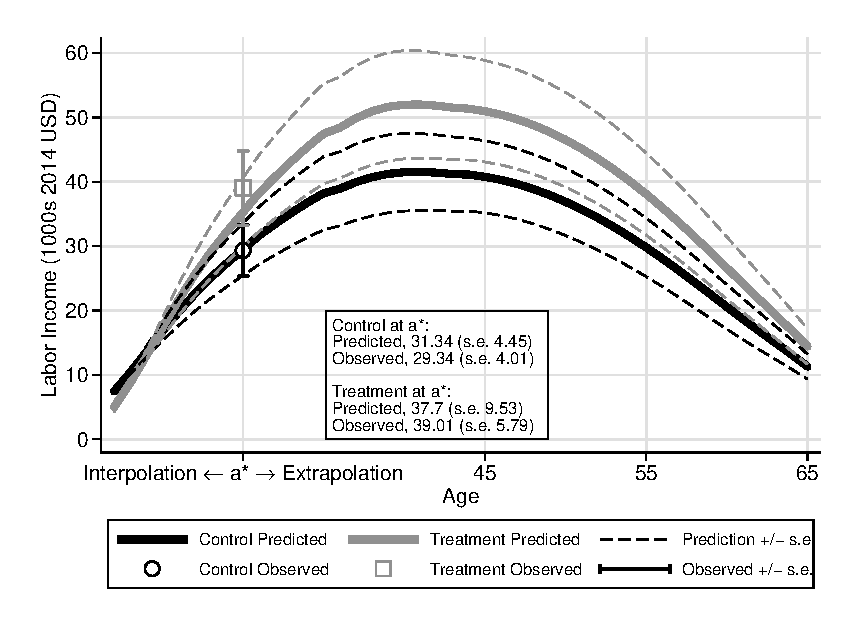
\includegraphics[width=\textwidth]{output/labor_25-65_pset1_mset1_male.eps}
\end{subfigure}%
\begin{subfigure}[h]{0.3\textwidth}
	\centering
	\caption{Post-treatment Variables, Males}
		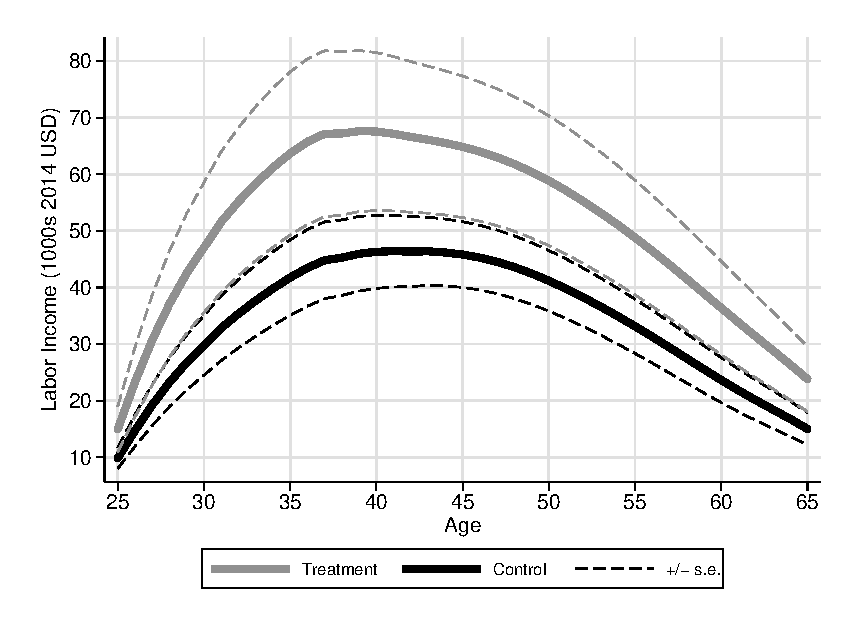
\includegraphics[width=\textwidth]{output/labor_25-65_pset1_mset2_male.eps}
\end{subfigure}%
\begin{subfigure}[h]{0.3\textwidth}
	\centering
	\caption{Pre- and Post-treatment Variables, Males}
		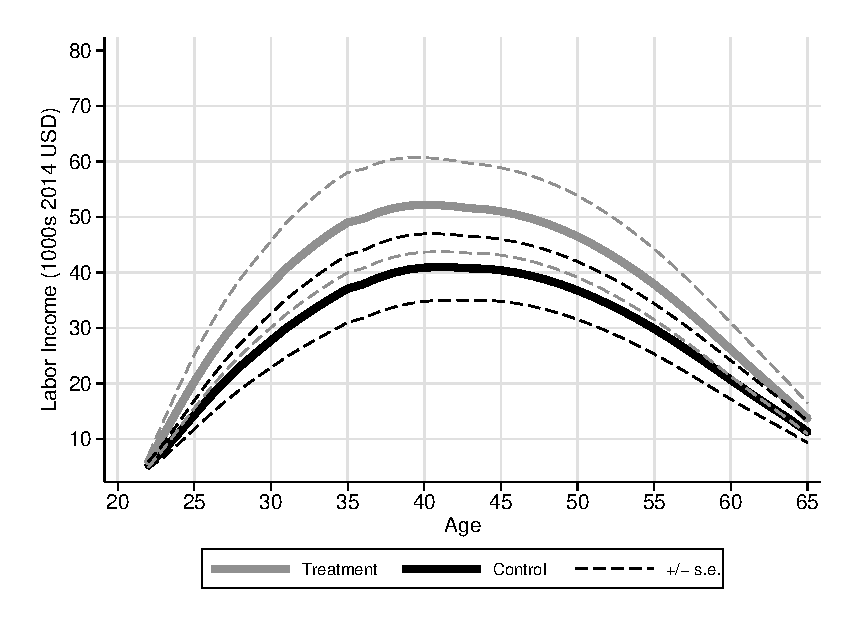
\includegraphics[width=\textwidth]{output/labor_25-65_pset1_mset3_male_sensitivity.eps}
\end{subfigure}
\footnotesize \justify
Note: This figure displays the predicted labor income profile obtained when constructing control- and treatment-group matches according to the procedure in Section~\ref{sec:necrosis}. We combine data from the Panel Study of Income Dynamics (PSID), the National Longitudinal Survey of Youth 1979 (NLSY79), and the Children of the National Longitudinal Survey of Youth 1979 (CNLSY79). We vary the matching variables across the different panels, for both males and females. Pre-treatment variables: male and black indicators and year of birth. Post-treatment variables: years of education at age 30 and labor income at age 30.
\end{sidewaysfigure}

\subsubsection{Containing Support}\label{app:containsupport}

\noindent We \textbf{assume containing support} between these auxiliary datasets and the analysis sample. This is required in order for us to reliably use external data to provide predictions for the ABC/CARE samples. Figure~\ref{fig:support} validates this assumption by displaying the overlapping support sets of ABC/CARE and our auxiliary data for the variables used to interpolate and extrapolate earnings.\footnote{For the male and black indicators, we do not provide evidence of containing support. All three non-experimental samples have vast numbers of males, females, and black individuals to cover the support in the experimental samples.}\\

\textbf{[JJH: Make sure this is cited in text. Make sure it's in display (as link) for Sage.]  [JLG: This is being mentioned in the text and it appears in Sage.]}

\begin{figure}[H]
		\caption{Support of ABC/CARE and Auxiliary Data} \label{fig:support}
	\begin{subfigure}[h]{0.8\textwidth}
	\centering
	\caption{Average PIAT Math Scores, Ages 5--7} \label{fig:support_math}
	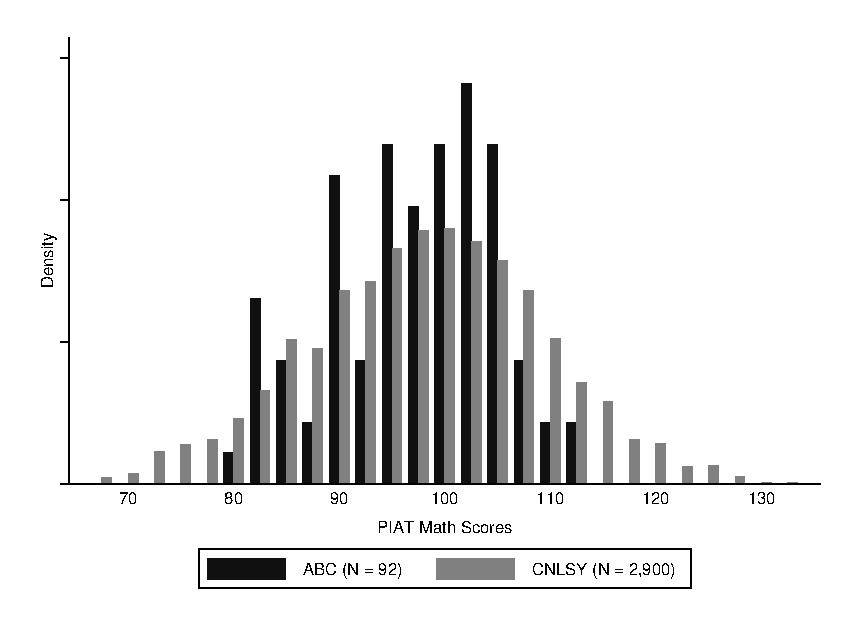
\includegraphics[width=\textwidth]{AppOutput/Methodology/support_math.eps}
	\end{subfigure}
	
	\begin{subfigure}[h]{0.8\textwidth}
	\centering
	\caption{Mother's Years of Education} \label{fig:support_meduc}
	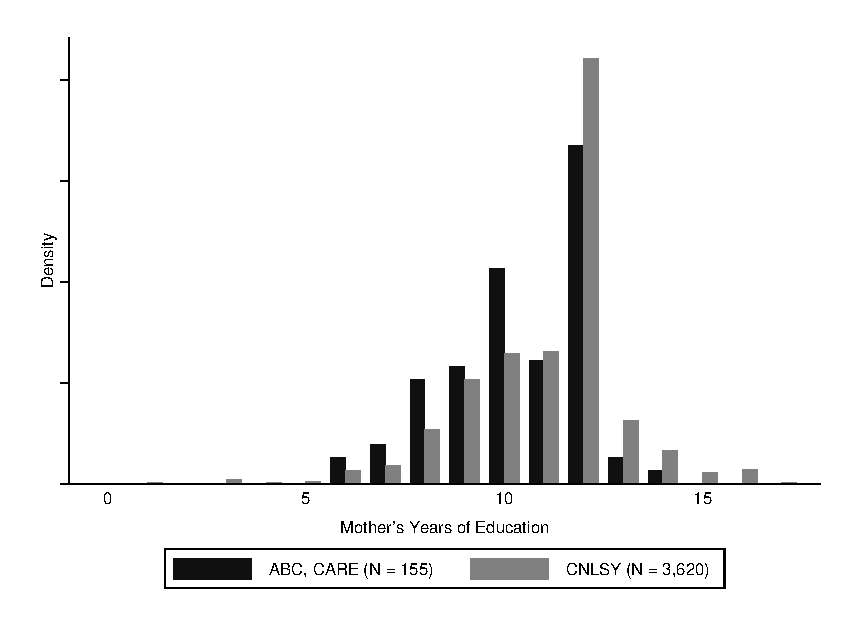
\includegraphics[width=\textwidth]{AppOutput/Methodology/support_momed.eps}
	\end{subfigure}
	
	\floatfoot{
	\footnotesize
	\noindent Note: These graphs display the support of ABC, PSID, NLSY79, and CNLSY
	for variables we use to project future earnings. PIAT math
	scores are averaged over ages 5--7.
	}
\end{figure}

\begin{figure}[H]
		\ContinuedFloat
	\begin{subfigure}[h]{0.8\textwidth}
	\centering
	\caption{Subject's Years of Education} \label{fig:support_educ}
	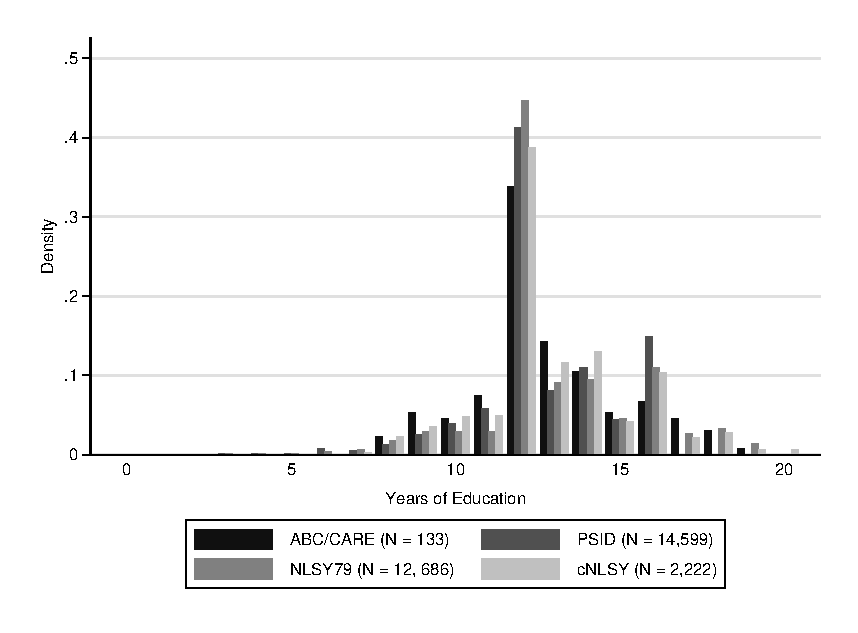
\includegraphics[width=\textwidth]{AppOutput/Methodology/support_educ.eps}
	\end{subfigure}
	
	\begin{subfigure}[h]{0.8\textwidth}
	\centering
	\caption{Income at Age 21} \label{fig:support_inc21}
	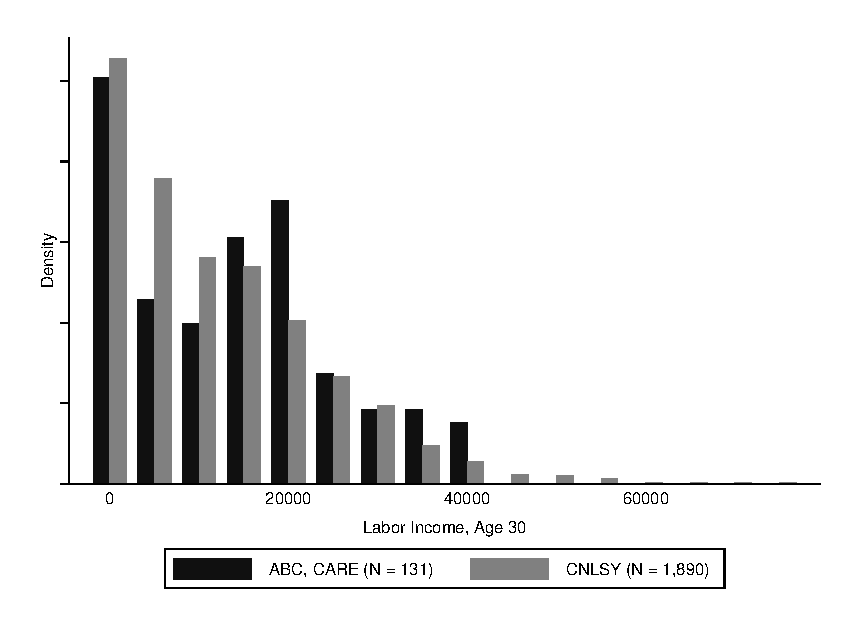
\includegraphics[width=\textwidth]{AppOutput/Methodology/support_inc21.eps}
	\end{subfigure}
	
\end{figure}

\begin{figure}[H]
	\ContinuedFloat
	
	\begin{subfigure}[h]{0.8\textwidth}
	\centering
	\caption{Income at Age 30} \label{fig:support_inc30}
	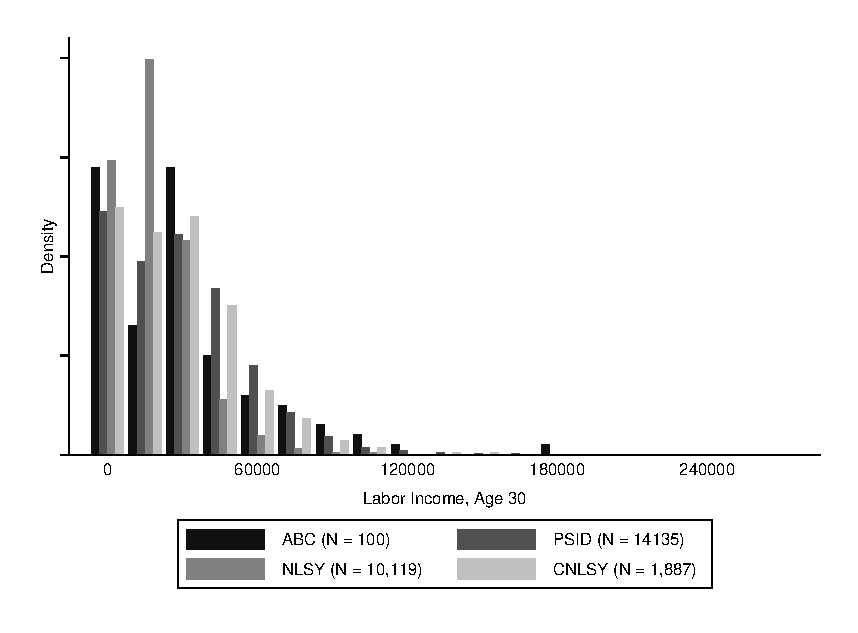
\includegraphics[width=\textwidth]{AppOutput/Methodology/support_inc30.eps}
	\end{subfigure}

	
	\begin{subfigure}[h]{0.8\textwidth}
	\centering
	\caption{Body Mass Index, Age 34} \label{fig:support_bmi}
	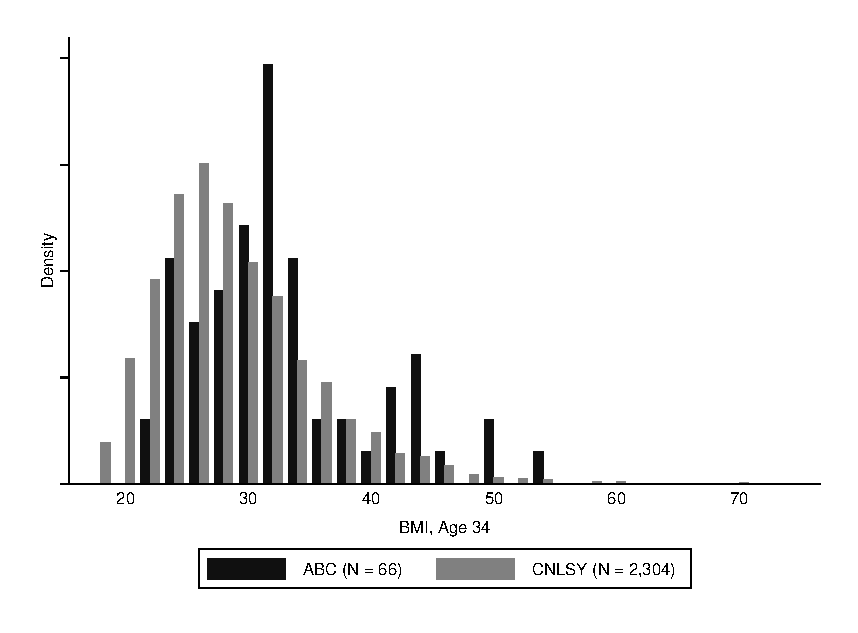
\includegraphics[width=\textwidth]{AppOutput/Methodology/support_bmi.eps}
	\end{subfigure}
	
\end{figure}

\subsubsection{Predictive Power} \label{appendix:pred}

\noindent We present evidence on the predictive power of the predictor variables, in both the control and treatment synthetic groups we construct in the PSID, NLSY79, and CNLSY. Tables~\ref{table:predpsid} to \ref{table:predcnlsy} show that, in each of the auxiliary samples that we use, the prediction variables $\bm{X}_{t}, \bm{B}$ are strong predictors of labor income at age 30. We present this evidence at age 30 both for brevity and to compare the predictive power of $\bm{X}_{t},\bm{B}$ on the outcomes we consider in the ABC/CARE sample. Analogous specification for the ABC/CARE sample are in Tables~\ref{table:predfac1} to \ref{table:predfac3}.\\

\begin{sidewaystable}[H]
\begin{threeparttable}
\caption{Predictors of Labor Income at Age 30, PSID}
\label{table:predpsid}
\centering
\footnotesize
\begin{tabular}{lccc} \toprule
 & (1) & (2) & (3) \\ \midrule
Male & 19,877.340*** & 20,336.227*** & 7,686.820*** \\
 & (404.768) & (390.549) & (411.552) \\
Black & -9,761.792*** & -6,406.807*** & -1,793.755*** \\
 & (385.350) & (362.171) & (299.889) \\
Education (30)  &  & 4,109.973*** & 1,619.779*** \\
 &  & (91.929) & (92.105) \\
Labor Income (28) &  &  & 0.741*** \\
 &  &  & (0.014) \\
Cons & 23,953.099*** & -30,187.589*** & -14,016.536*** \\
 & (289.118) & (1,167.401) & (1,080.036) \\
 &  &  &  \\ \\ \midrule
Observations & 14,979 & 13,908 & 9,812 \\
$R^2$ & 0.172 & 0.291 & 0.657 \\ \bottomrule
\end{tabular}

\begin{tablenotes}
\footnotesize
\item Note: All columns display regressions of labor income at age 30 on the different variables listed in the rows. If the space for the coefficient appears empty, it was not included in the regression. All money figures are in 2014 USD. The parentheses next to the variable indicates the age of measurement. Education is measured as years of education. Robust standard errors are in parentheses. We weigh the individuals in the PSID to match them on observed characteristics to the individuals using the procedure in Section~\ref{sec:necrosis} based on male and black indicators, year of birth, years of education at age 30, and labor income at age 30 to find synthetic control and treatment groups in the PSID. $^{***}$: $p$-value $< .01$. $^{**}$: $p$-value $< .05$. $^{*}$: $p$-value $< .10$.
\end{tablenotes}
\end{threeparttable}
\end{sidewaystable}

\begin{sidewaystable}[H]
\begin{threeparttable}
\caption{Predictors of Labor Income at Age 30, NLSY79}
\label{table:prednlsy}
\centering
\footnotesize
\begin{tabular}{lcccccccc} \toprule
 & (1) & (2) & (3) & (4) & (5) & (6) & (7) & (8) \\
 Group Matched & Control & Treatment & Control & Treatment & Control & Treatment & Control & Treatment \\ \midrule
Male & 6,219.175*** & 6,356.307*** & 7,117.820*** & 7,607.672*** & 5,725.956*** & 6,216.821*** & 2,106.570*** & 2,311.490*** \\
 & (381.462) & (444.690) & (352.939) & (407.219) & (364.544) & (425.777) & (265.712) & (303.553) \\
Black & -5,607.642*** & -5,688.084*** & -5,150.394*** & -4,994.999*** & -3,823.029*** & -3,775.318*** & -1,737.614*** & -1,621.612*** \\
 & (386.635) & (439.804) & (356.854) & (399.225) & (381.924) & (431.636) & (256.122) & (287.850) \\
Education (30) &  &  & 2,536.795*** & 2,634.281*** & 2,593.961*** & 2,706.537*** & 799.974*** & 773.933*** \\
 &  &  & (81.757) & (95.205) & (85.765) & (100.476) & (73.768) & (79.358) \\
Labor Income (21) &  &  &  &  & 0.637*** & 0.627*** &  &  \\
 &  &  &  &  & (0.043) & (0.050) &  &  \\
Labor Income (28) &  &  &  &  &  &  & 0.774*** & 0.782*** \\
 &  &  &  &  &  &  & (0.021) & (0.022) \\
Constant & 15,572.398*** & 16,568.877*** & -17,659.060*** & -18,893.301*** & -21,611.129*** & -22,998.860*** & -5,761.074*** & -5,570.719*** \\
 & (304.541) & (336.484) & (1,085.558) & (1,274.381) & (1,148.548) & (1,366.048) & (834.721) & (959.266) \\ \\ \midrule Observations & 7,297 & 5,874 & 7,297 & 5,874 & 6,650 & 5,291 & 6,601 & 5,324 \\
$R^2$ & 0.102 & 0.095 & 0.245 & 0.250 & 0.309 & 0.305 & 0.690 & 0.693 \\ \hline
\end{tabular}

\begin{tablenotes}
\footnotesize
\item Note: All columns display regressions of labor income at age 30 on the different variables listed in the rows. If the space for the coefficient appears empty, it was not included in the regression. All money figures are in 2014 USD. The parentheses next to the variable indicates the age of measurement. Education is measured as years of education. Robust standard errors are in parentheses. We weigh the individuals in the NLSY79 to match them on observed characteristics to the individuals using the procedure in Section~\ref{sec:necrosis} based on male and black indicators, year of birth, years of education at age 30, and labor income at age 30 to find synthetic control and treatment groups in the NLSY79. $^{***}$: $p$-value $< .01$. $^{**}$: $p$-value $< .05$. $^{*}$: $p$-value $< .10$.
\end{tablenotes}
\end{threeparttable}
\end{sidewaystable}

\begin{sidewaystable}[H]
\begin{threeparttable}
\caption{Predictors of Labor Income at Age 30, CNLSY}
\label{table:predcnlsy}
\centering
\footnotesize
\begin{tabular}{lcccccc} \toprule
 & (1) & (2) & (3) & (4) & (5) & (6) \\ 
Group Matched & Control & Treatment & Control & Treatment & Control & Treatment \\ \midrule
Male & 7,919.35*** & 7,755.32*** & 7,483.55*** & 7,472.02*** & 3,634.65*** & 3,740.61*** \\
 & (937.46) & (974.57) & (990.66) & (1,030.20) & (1,231.12) & (1,306.46) \\
Black  & -7,480.51*** & -7,721.48*** & -3,669.31*** & -3,799.02*** & -1,853.59 & -2,022.28* \\
 & (925.86) & (961.86) & (989.18) & (1,029.09) & (1,156.85) & (1,202.94) \\
Mother's Education & 1,888.32*** & 1,833.29*** & 303.02 & 288.90 & 284.94 & 235.17 \\
 & (258.71) & (271.05) & (293.84) & (309.08) & (357.69) & (393.81) \\
PIAT (5-7) &  &  & 168.64*** & 170.88*** & 169.51*** & 169.89** \\
 &  &  & (48.44) & (50.18) & (63.42) & (66.41) \\
Education (30)  &  &  & 3,678.09*** & 3,736.28*** & 2,223.04*** & 2,353.75*** \\
 &  &  & (250.08) & (264.84) & (434.21) & (457.65) \\
Labor Income (21) &  &  & 0.51*** & 0.50*** &  &  \\
 &  &  & (0.06) & (0.06) &  &  \\
BMI (34) &  &  & -45.78 & -48.11 & -174.13* & -183.16* \\
 &  &  & (70.83) & (72.79) & (96.27) & (100.26) \\
Labor Income (28) &  &  &  &  & 0.48*** & 0.46*** \\
 &  &  &  &  & (0.07) & (0.07) \\
Constant & 4,170.58 & 5,151.64* & -47,898.77*** & -48,608.54*** & -30,593.81*** & -31,042.44*** \\
 & (2,940.08) & (3,083.88) & (5,285.02) & (5,504.80) & (6,818.91) & (7,102.58) \\ \\ \midrule
 Observations & 1,880 & 1,876 & 1,463 & 1,459 & 734 & 733 \\ 
$R^2$ & 0.09 & 0.09 & 0.29 & 0.29 & 0.50 & 0.49 \\ \bottomrule
\end{tabular}

\begin{tablenotes}
\footnotesize
\item  Note: All columns display regressions of labor income at age 30 on the different variables listed in the rows. If the space for the coefficient appears empty, it was not included in the regression. All money figures are in 2014 USD. The parentheses next to the variable indicates the age of measurement. Education is measured as years of education. Robust standard errors are in parentheses. We weigh the individuals in the CNLSY to match them on observed characteristics to the individuals using the procedure in Section~\ref{sec:necrosis} based on male and black indicators, year of birth, years of education at age 30, and labor income at age 30 to find synthetic control and treatment groups in the CNLSY. $^{***}$: $p$-value $< .01$. $^{**}$: $p$-value $< .05$. $^{*}$: $p$-value $< .10$.
\end{tablenotes}
\end{threeparttable}
\end{sidewaystable}

\subsubsection{Sensitivity Analysis}

\noindent We examine the sensitivity of our predictions to the choice of different prediction variables. We reproduce three exercises to analyze this for labor income: (i) our baseline prediction, which is based on $\bm{X}_{t}, \bm{B}$ and the lagged value of the predicted labor income, i.e. at time $t$ we base the prediction on $\bm{X}_{t}, \bm{B}$ and (predicted) labor income at $t-1$; (ii) the same as (i) but without using $\bm{B}$; (iii) the same as (i) but without using $\bm{X}_{t}$.\\

\noindent Figure~\ref{fig:predictsensitivity} displays this exercise. Any prediction based on $\bm{X}_{t}$ produces labor income profiles with significant differences between the treatment and control groups, especially for males. Adding background variables $\bm{B}$ do not help distinguish treatment and control group (as expected given balance at baseline).

\textbf{[JJH: Jorge, this repeats.] [JLG: Professor, C.4.6. is sensitivity to using different variables to predict. C.4.3.1 is sensitivity to different variables to construct the matching. ]}

\begin{sidewaysfigure}[H]
\centering
\caption{Predicted Labor Income Profiles, Varying the Predictor Variables}\label{fig:predictsensitivity}
\begin{subfigure}[h]{0.3\textwidth}
		\centering
		\caption{Lagged Labor Income and $\bm{B}$, Females}
		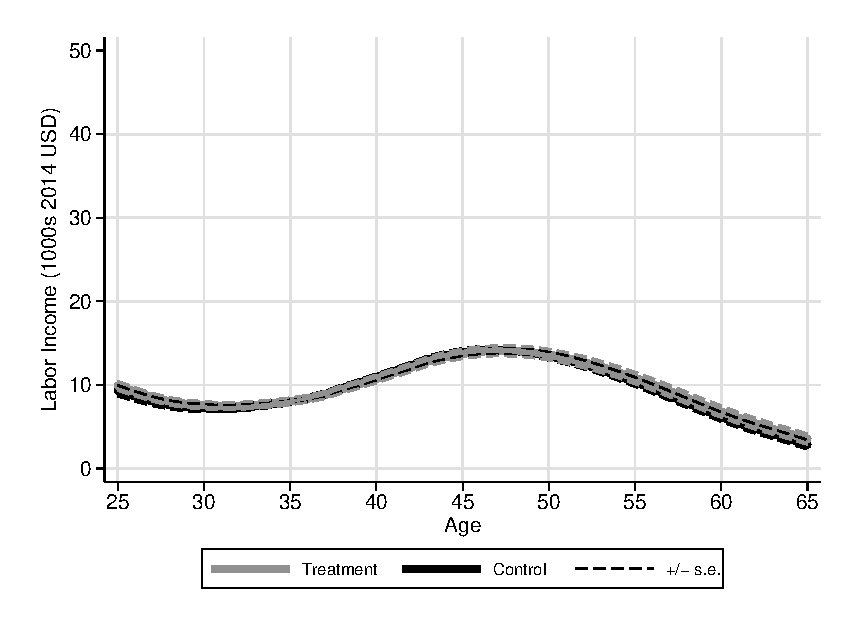
\includegraphics[width=\textwidth]{output/labor_25-65_pset3_mset3_female.eps}
\end{subfigure}%
\begin{subfigure}[h]{0.3\textwidth}
	\centering
	\caption{Lagged Labor Income and $\bm{X}_{t}$, Females}
		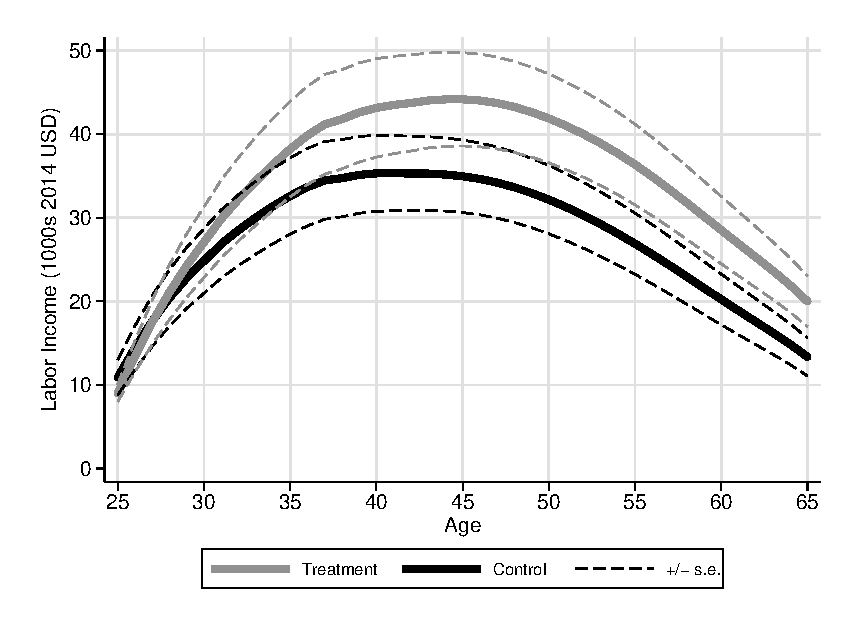
\includegraphics[width=\textwidth]{output/labor_25-65_pset6_mset3_female.eps}
\end{subfigure}%
\begin{subfigure}[h]{0.3\textwidth}
	\centering
	\caption{Lagged Labor Income and $\bm{B}, \bm{X}_{t}$, Females}
		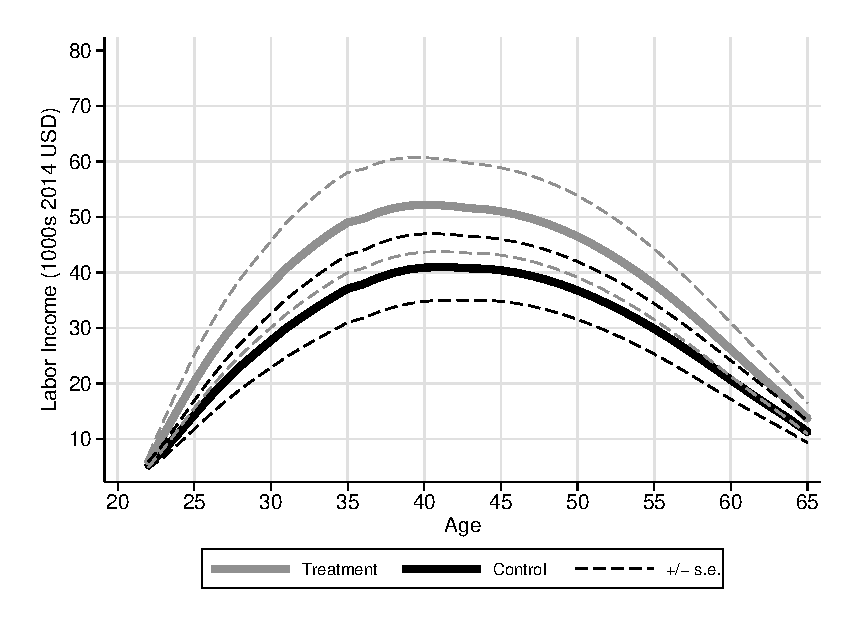
\includegraphics[width=\textwidth]{output/labor_25-65_pset1_mset3_male_sensitivity.eps}
\end{subfigure}
\begin{subfigure}[h]{0.3\textwidth}
		\centering
		\caption{Lagged Labor Income and $\bm{B}$, Males}
		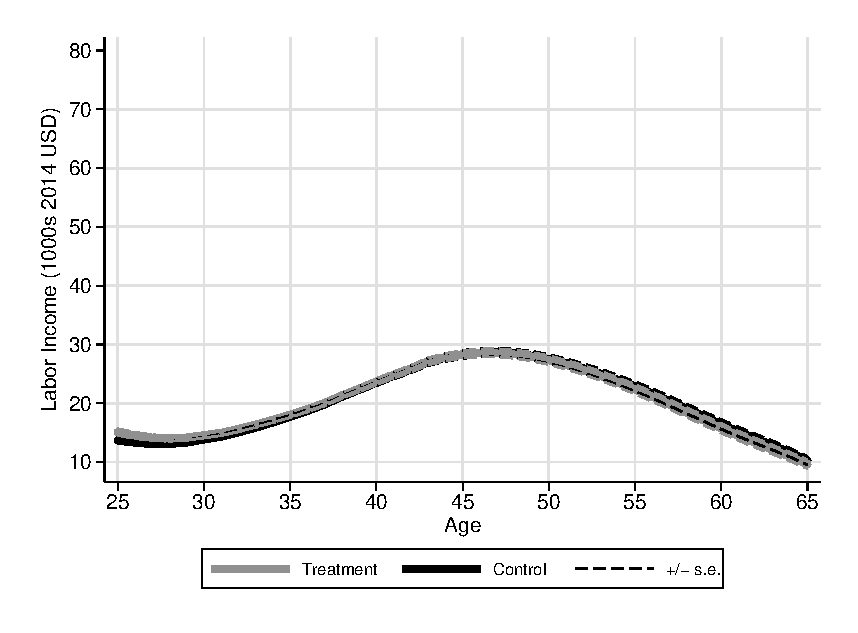
\includegraphics[width=\textwidth]{output/labor_25-65_pset3_mset3_male.eps}
\end{subfigure}%
\begin{subfigure}[h]{0.3\textwidth}
	\centering
	\caption{Lagged Labor Income and $\bm{X}_{t}$, Males}
		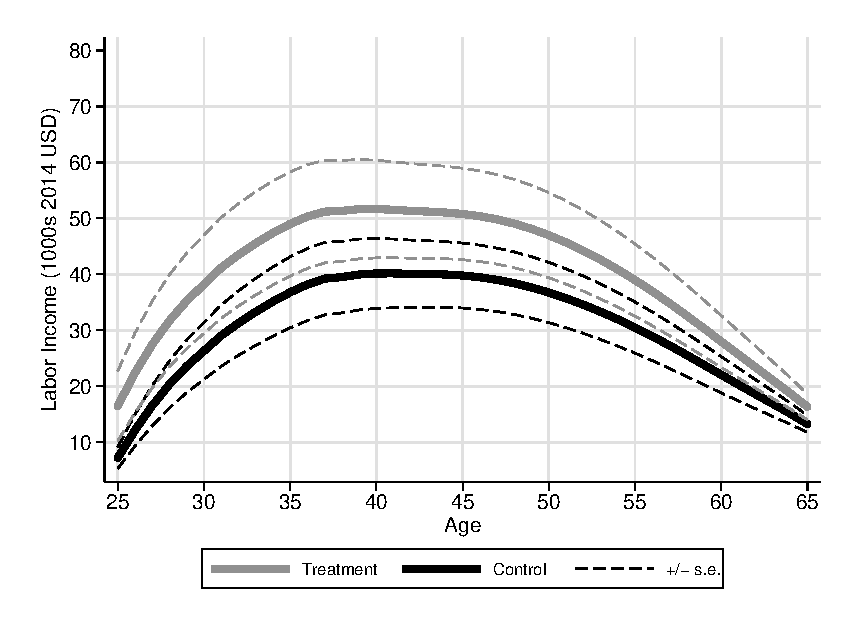
\includegraphics[width=\textwidth]{output/labor_25-65_pset6_mset3_male.eps}
\end{subfigure}%
\begin{subfigure}[h]{0.3\textwidth}
	\centering
	\caption{Lagged Labor Income and $\bm{B}, \bm{X}_{t}$, Males}
		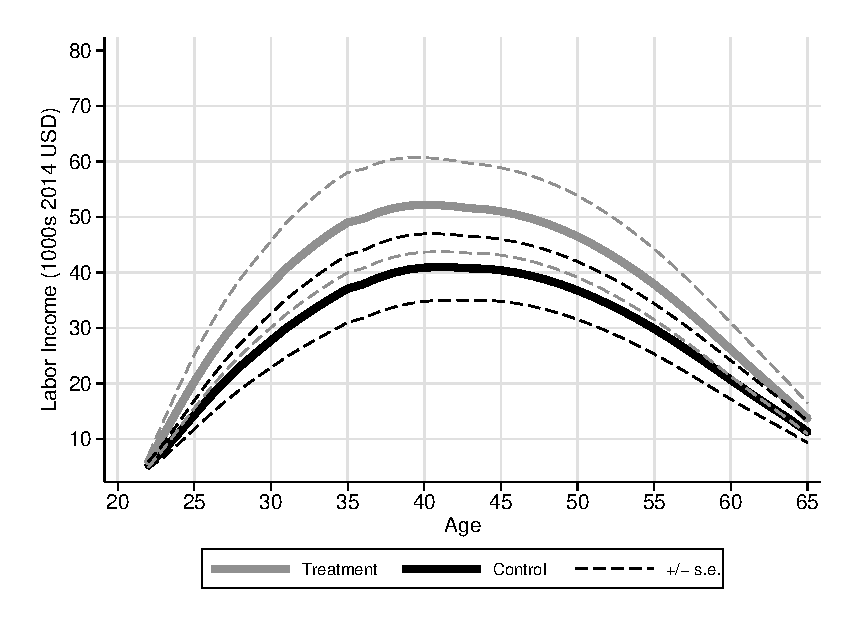
\includegraphics[width=\textwidth]{output/labor_25-65_pset1_mset3_male_sensitivity.eps}
\end{subfigure}
\footnotesize \justify
Note: This figure displays the predicted labor income profile obtained when constructing control- and treatment-group matches according to the procedure in Section~\ref{sec:necrosis}. We combine data from the Panel Study of Income Dynamics (PSID), the National Longitudinal Survey of Youth 1979 (NLSY79), and the Children of the National Longitudinal Survey of Youth 1979 (CNLSY79). We vary the prediction variables across the different panels, for both males and females. $\bm{B}$ variables: male and black indicators, and mother's education. $\bm{X}_{t}$ variables: years of education at age 30, labor income at ages 21 and 30, and BMI at age 34.
\end{sidewaysfigure}

\subsection{Testing  Assumption~\ref{ass:eczema}} \label{app:invariance}

\noindent In this section we test Assumption~\ref{ass:eczema} in the main text. Under Assumption~\ref{ass:eczema}, our empirical predictions are based on the null hypothesis:

\begin{equation}
\phi_{j,t}^0 \left( \bm{X}_{t}^d, \bm{B}, \varepsilon_{j,t}^d\right) = \phi_{j,t}^1 \left( \bm{X}_{t}^d, \bm{B}, \bm{\varepsilon}_{j,t}^d\right) \label{eq:eqs}
\end{equation}

\noindent at time $t \in \{0, \ldots, T\}$ and for outcome $j \in \mathcal{J}_{t}$.\\

\noindent In our empirical analysis, we assume that $\phi_{j,t}^d$ is a linear function of $ \bm{X}_{t}^d, \bm{B}, \bm{\varepsilon}_{j,t}^d$ for $d \in \{0,1\}$. We test if the coefficients characterizing $\phi_{j,t}^d$ are the same for specifications including (i) $\bm{X}_{t}^d$, (ii) including  $\bm{B}$, and (iii) $\bm{X}_{t}^d, \bm{B}$. For this test, we use the two outcomes we predict, labor income and transfer income.\footnote{We observe both variables at age 30 in the ABC/CARE sample, which we use to test the assumption.}

\noindent A potential problem is endogeneity (e.g., mean dependence between schooling years and unobserved skills). Unless the bias in the treatment and control groups are exactly the same, endogeneity would bias our forecasts. A sufficient condition to obtain unbiased forecasts is $\mathbb{E} \left[ \bm{\varepsilon}_{j,t}^0 | \bm{X}_{t}^d, \bm{B} \right] = \mathbb{E} \left[ \bm{\varepsilon}_{j,t}^1 | \bm{X}_{t}^d, \bm{B} \right]$.\\

\noindent An alternative is to follow \citet{Heckman_Pinto_etal_2013_PerryFactor} and obtain an approximation for  $\bm{\varepsilon}_{j,t}^d$ based on a measurement system. Formally, let the system be

\begin{eqnarray}
\bm{M}_{t}^d     &=& \bm{\lambda}^d \bm{\theta}_{t}^d +  \bm{\upsilon}_t^d, \text{ where } \bm{\theta}^d  \independent \bm{\upsilon}_{t}^d \ \forall t \\ \nonumber
\bm{\varepsilon}_{t}^d &=& \bm{\beta}^d \bm{\theta}_{t}^d + \bm{\omega}_{t}^d \text{ where } \bm{\theta}^d  \independent \bm{\omega}_{t}^d \ \forall t \\ \nonumber
&\upsilon_{t}^d \independent \omega_{t}^d.
\label{eq:msystem}
\end{eqnarray}

\noindent With an auxiliary system of measures such that $\bm{M}_{t}^d $ has at least three elements, we are able to identify the vectors of coefficients characterizing these system: $\bm{\lambda}^d, \bm{\beta}^d$, as well as the respective covariance matrices $\Sigma_{\bm{\theta}_{t}^d}, \Sigma_{\bm{\upsilon}_{t}^d}$, and use the method in \citet{Bartlett_1938_Nature} to obtain an estimate of $\bm{\theta}_{t}^d$ \citep{Cunha_Heckman_ea_2005_oep,Cunha_Heckman_etal_2010_est_tech_cognoncog}. To put this in practice, we assume that $\bm{\theta}_{t}^d$ has two dimensions (one representing cognitive skill and another representing non-cognitive skill). We assume dedicated measures for these skills at one time period. Put simply, we have two independent systems, one to measure $\theta_{c}^d$ and one to measure $\theta_{n}^d$, where $\bm{\theta}_{t}^d: = \left[ \theta_{c}^d, \theta_{n}^d \right]$. Further, we assume a common measurement system for the treatment and control groups (this is a sensible assumption given the small size of our sample). This assumption implies that $\bm{\lambda}^d, \bm{\beta}^d$, as well as $\bm{\Sigma}_{\bm{\theta}_{t}^d}, \bm{\Sigma}_{\bm{\upsilon}_{t}^d}$ are the same either when $d = 0$ or when $d = 1$.\\

\noindent We use a set of measures from ages 2 to 8 to to obtain an estimate of $\theta_{c}^d$ and a set of measures of somatization, hostility, depression, and global index of mental health to measure (all at age 21) to estimate $\theta_{n}^d$.\footnote{For definitions and treatment effects on these variables see Appendix~\ref{appendix:results}.}\\

\noindent Given Condition~\eqref{eq:msystem}, the estimated coefficients characterizing \eqref{eq:eqs} are unbiased, and therefore our tests are valid. For each specification we consider, we present results controlling and not controlling for estimates of $\bm{\theta}_{t}^d$. Figure~\ref{figure:factors} presents the distribution of estimates for the two dimensions of $\bm{\theta}_{t}^d$ that we consider and Tables~\ref{table:predfac1} to \ref{table:predfacti3} present estimates of the two functions in \eqref{eq:eqs} using different specifications and the different outcomes. There is no strong evidence to reject the null hypotheses implied by the equality in \eqref{eq:eqs}.


\begin{figure}[H]
\centering
\caption{Estimates of Cognitive ($\theta_{c}^d$) and Non-cognitive Skills ($\theta_{n}^d$)}\label{figure:factors}
\begin{subfigure}[h]{0.7\textwidth}
		\centering
		\caption{Cognitive} \label{fig:c}
		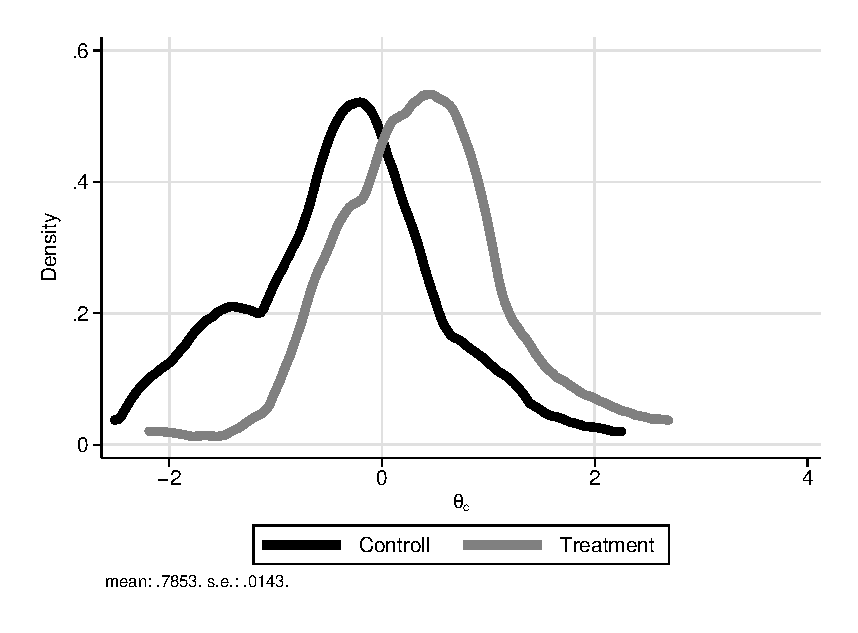
\includegraphics[width=\textwidth]{output/abccare_cfactor.eps}
\end{subfigure}

\begin{subfigure}[h]{0.7\textwidth}
	\centering
	\caption{Non-cognitive} \label{fig:n}
		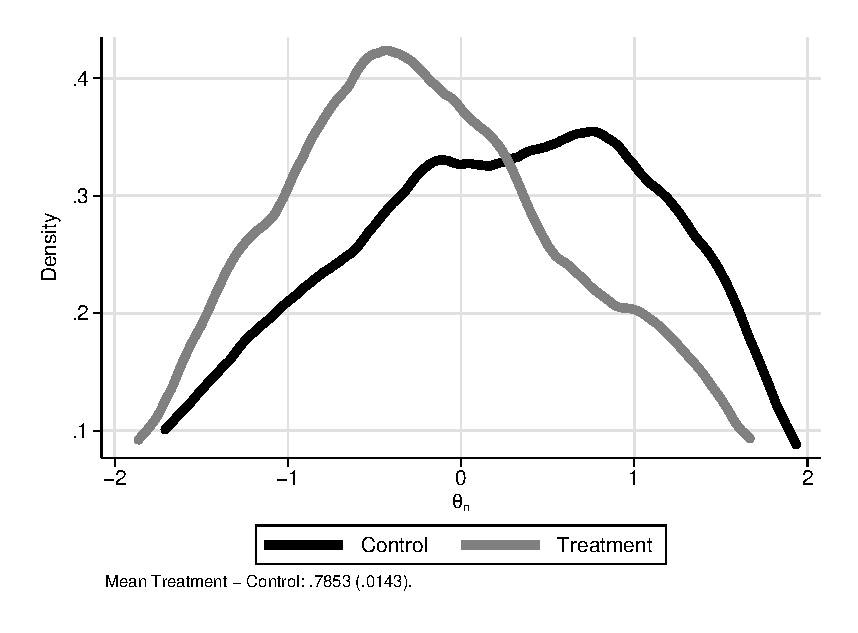
\includegraphics[width=\textwidth]{output/abccare_nfactor.eps}
\end{subfigure}
\footnotesize \justify
Note: Panels (a) displays a factor score estimated based on the measurement system in \eqref{eq:msystem} and measures of IQ at ages 2, 3, 4, 5, 7, and 8 (cognitive skill). Panel (b) displays an analogous exercise using measures measures of somatization, hostility, depression, and a global mental health index at age 21 (non-cognitive skill). Both measures of skills are standardized to a mean of $0$ and a standard deviation of $1$. The mean difference between treatment and control is displayed below each panel, with standard error in parentheses. Standard errors are based on the bootstrap empirical distribution.
\end{figure}

\begin{sidewaystable}[H]
\begin{threeparttable}
\caption{Prediction of Labor Income at Age 30 Accounting for $\bm{B}$ and $\bm{\theta}$, ABC/CARE}
\label{table:predfac1}
\centering
\footnotesize
\begin{tabular}{lcccccccccccc} \toprule
&\multicolumn{2}{c}{Control} & \multicolumn{2}{c}{Treatment} & \multicolumn{2}{c}{Treatment - Control} & \multicolumn{2}{c}{Control} & \multicolumn{2}{c}{Treatment} & \multicolumn{2}{c}{Treatment - Control} \\
 & Coefficient  & $p$-value  & Coefficient  & $p$-value & Coefficient  & $p$-value  & Coefficient  & $p$-value  & Coefficient  & $p$-value  & Coefficient  & $p$-value \\ \midrule
Mother's Education &   440.383 &     0.380 &  3,693.417 &     0.300 &  3,253.033 &     0.340 &  -203.428 &     0.525 &  3,328.924 &     0.375 &  3,532.352 &     0.370 \\  
PIAT (5-7) &         &         &         &         &         &         &         &         &         &         &         &         \\
Education (30) &         &         &         &         &         &         &         &         &         &         &         &         \\
Labor Income (21) &         &         &         &         &         &         &         &         &         &         &         &         \\
BMI (34) &         &         &         &         &         &         &         &         &         &         &         &         \\
$\hat{\bm{\theta}}_{c}$ &         &         &         &         &         &         &  1,322.009 &     0.360 &  -329.080 &     0.510 & -1,651.089 &     0.535 \\  
$\hat{\bm{\theta}}_{n}$ &         &         &         &         &         &         &   947.122 &     0.445 &  9,979.087 &     0.195 &  9,031.964 &     0.205 \\  
Constant  & 24,500.00 &     0.130 &  3,731.899 &     0.475 & -20,700.00 &     0.610 & 30,700.00 &     0.120 &  8,791.943 &     0.475 & -21,900.00 &     0.600 \\  
\bottomrule \end{tabular}

\begin{tablenotes}
\footnotesize
\item Note: Prediction of labor income at age 30 based on the variables listed in the row. Empty cells indicate that the variable was not used in the prediction. For each coefficient we provide point estimate and $p$-value for the treatment and control groups and a test for the treatment-control difference. $\hat{\theta}_{c}$: factor score estimated based on the measurement system in \eqref{eq:msystem} and measures of IQ at ages 2, 3, 4, 5, 7, and 8 (cognitive skill). $\hat{\theta}_{n}$: factor score estimated based on the measurement system in \eqref{eq:msystem} and measures of somatization, hostility, depression, and a global mental health index at age 21 (non-cognitive skill). Both measures of skills are standardized to a mean of $0$ and a standard deviation of $1$. Inference is based on the empirical bootstrap distribution. If the estimates for the constant terms are in the ten or hundred thousands, we report a figure that has been rounded to the thousands.
\end{tablenotes}
\end{threeparttable}
\end{sidewaystable}

\begin{sidewaystable}[H]
\begin{threeparttable}
\caption{Prediction of Labor Income at Age 30 Accounting for $\bm{\theta}, \bm{X}_{t} \text{ (set 1)}$, ABC/CARE}
\label{table:predfac2}
\centering
\footnotesize
\begin{tabular}{lcccccccccccc} \toprule
&\multicolumn{2}{c}{Control} & \multicolumn{2}{c}{Treatment} & \multicolumn{2}{c}{Treatment - Control} & \multicolumn{2}{c}{Control} & \multicolumn{2}{c}{Treatment} & \multicolumn{2}{c}{Treatment - Control} \\ \midrule
 & Coefficient  & $p$-value  & Coefficient  & $p$-value & Coefficient  & $p$-value  & Coefficient  & $p$-value  & Coefficient  & $p$-value  & Coefficient  & $p$-value \\ \midrule
Mother's Education & -1185.376 &     0.760 &  4920.358 &     0.220 &  6105.733 &     0.170 & -1593.767 &     0.795 &  7869.586 &     0.250 &  9463.354 &     0.180 \\  
PIAT (5-7) &   152.554 &     0.325 &  -576.029 &     0.680 &  -728.583 &     0.730 &   349.690 &     0.310 &  -948.807 &     0.735 & -1298.497 &     0.815 \\  
Education (30)  &  2956.656 &     0.015 & 10915.656 &     0.025 &  7959.000 &     0.060 &  4952.654 &     0.015 & 12374.844 &     0.025 &  7422.189 &     0.120 \\  
Labor Income (21) &     0.679 &     0.030 &    -0.465 &     0.710 &    -1.144 &     0.895 &     1.056 &     0.030 &    -0.899 &     0.755 &    -1.955 &     0.930 \\  
BMI (34) &        &        &        &        &        &        &        &        &        &        &        &         \\
$\theta_{c}$ &        &        &        &        &        &        &   349.690 &     0.310 &  -948.807 &     0.735 & -1298.497 &     0.815 \\  
$\theta_{n}$ &        &        &        &        &        &        &  4952.654 &     0.015 & 12374.844 &     0.025 &  7422.189 &     0.120 \\  
Constant &   152.554 &     0.325 &  -576.029 &     0.680 &  -728.583 &     0.730 &     1.056 &     0.030 &    -0.899 &     0.755 &    -1.955 &     0.930 \\  
\bottomrule \end{tabular}
\begin{tablenotes}
\footnotesize
\item Note: Prediction of labor income at age 30 based on the variables listed in the row. Empty cells indicate that the variable was not used in the prediction. For each coefficient we provide point estimate and $p$-value for the treatment and control groups and a test for the treatment-control difference. $\hat{\theta}_{c}$: factor score estimated based on the measurement system in \eqref{eq:msystem} and measures of IQ at ages 2, 3, 4, 5, 7, and 8 (cognitive skill). $\hat{\theta}_{n}$: factor score estimated based on the measurement system in \eqref{eq:msystem} and measures of somatization, hostility, depression, and a global mental health index at age 21 (non-cognitive skill). Both measures of skills are standardized to a mean of $0$ and a standard deviation of $1$. Inference is based on the empirical bootstrap distribution. If the estimates for the constant terms are in the ten or hundred thousands, we report a figure that has been rounded to the thousands.
\end{tablenotes}
\end{threeparttable}
\end{sidewaystable}

\begin{sidewaystable}[H]
\begin{threeparttable}
\caption{Prediction of Labor Income at Age 30 Accounting for $\bm{B}$ and $\bm{\theta}, \bm{X}_{t} \text{ (set 2)}$, ABC/CARE}
\label{table:predfac3}
\centering
\footnotesize
\begin{tabular}{lcccccccccccc} \toprule
&\multicolumn{2}{c}{Control} & \multicolumn{2}{c}{Treatment} & \multicolumn{2}{c}{Treatment - Control} & \multicolumn{2}{c}{Control} & \multicolumn{2}{c}{Treatment} & \multicolumn{2}{c}{Treatment - Control} \\
 & Coefficient  & $p$-value  & Coefficient  & $p$-value & Coefficient  & $p$-value  & Coefficient  & $p$-value  & Coefficient  & $p$-value  & Coefficient  & $p$-value \\ \midrule
Mother's Education & -3,396.557 &     0.905 &  -595.010 &     0.570 &  2,801.547 &     0.265 & -4,939.547 &     0.925 & -1,783.446 &     0.645 &  3,156.101 &     0.300 \\  
PIAT (5-7)&   646.297 &     0.100 &   213.484 &     0.395 &  -432.812 &     0.645 &  1,252.342 &     0.035 &   290.428 &     0.450 &  -961.914 &     0.745 \\  
Education (30) &  2,171.877 &     0.170 & 18,933.859 &     0.000 & 16,761.982 &     0.020 &  4,919.624 &     0.110 & 20,676.168 &     0.010 & 15,756.545 &     0.035 \\  
Labor Income (21) &     0.606 &     0.080 &     0.316 &     0.230 &    -0.290 &     0.645 &     0.701 &     0.195 &     0.131 &     0.360 &    -0.569 &     0.680 \\  
BMI (34)  &  -167.372 &     0.620 & -1,177.142 &     0.980 & -1,009.770 &     0.920 &   292.583 &     0.310 & -1,078.149 &     0.970 & -1,370.732 &     0.910 \\  
$\hat{\theta}_{c}$ &         &        &        &        &        &        &-6,549.362 &     0.805 &  -127.975 &     0.500 &  6,421.387 &     0.350 \\  
$\hat{\theta}_{n}$ &         &        &        &        &        &        & 3,708.096 &     0.340 &  3,817.413 &     0.250 &   109.317 &     0.500 \\  
Constant & -28,600.00 &     0.760 & -192,000.00 &     0.970 & -163,000.00 &     0.915 & -120,000.00 &     0.925 & -213,000.00 &     0.915 & -92,500.00 &     0.710 \\  
\bottomrule \end{tabular}

\begin{tablenotes}
\footnotesize
\item Note: Prediction of labor income at age 30 based on the variables listed in the row. Empty cells indicate that the variable was not used in the prediction. For each coefficient we provide point estimate and $p$-value for the treatment and control groups and a test for the treatment-control difference. $\hat{\theta}_{c}$: factor score estimated based on the measurement system in \eqref{eq:msystem} and measures of IQ at ages 2, 3, 4, 5, 7, and 8 (cognitive skill). $\hat{\theta}_{n}$: factor score estimated based on the measurement system in \eqref{eq:msystem} and measures of somatization, hostility, depression, and a global mental health index at age 21 (non-cognitive skill). Both measures of skills are standardized to a mean of $0$ and a standard deviation of $1$. Inference is based on the empirical bootstrap distribution. If the estimates for the constant terms are in the ten or hundred thousands, we report a figure that has been rounded to the thousands.
\end{tablenotes}
\end{threeparttable}
\end{sidewaystable}

\begin{sidewaystable}[H]
\begin{threeparttable}
\caption{Prediction of Transfer Income at Age 30 Accounting for $\bm{B}$ and $\bm{\theta}$, ABC/CARE}
\label{table:predfac1}
\centering
\footnotesize
\begin{tabular}{lcccccccccccc} \toprule
&\multicolumn{2}{c}{Control} & \multicolumn{2}{c}{Treatment} & \multicolumn{2}{c}{Treatment - Control} & \multicolumn{2}{c}{Control} & \multicolumn{2}{c}{Treatment} & \multicolumn{2}{c}{Treatment - Control} \\
 & Coefficient  & $p$-value  & Coefficient  & $p$-value & Coefficient  & $p$-value  & Coefficient  & $p$-value  & Coefficient  & $p$-value  & Coefficient  & $p$-value \\ \midrule
Mother's Education  &  -360.538 &     0.775 &  -354.602 &     0.760 &     5.936 &     0.500 &  -468.425 &     0.810 &  -553.713 &     0.735 &   -85.288 &     0.545 \\  
PIAT (5-7) &         &         &         &         &         &         &         &         &         &         &         &         \\  
Education (30) &         &         &         &         &         &         &         &         &         &         &         &         \\  
Labor Income (21)  &         &         &         &         &         &         &         &         &         &         &         &         \\  
BMI (34) &         &         &         &         &         &         &         &         &         &         &         &         \\  
$\hat{\theta}_{c}$ &         &         &         &         &         &         &  -436.325 &     0.740 &   -46.354 &     0.510 &   389.971 &     0.300 \\  
$\hat{\theta}_{n}$ &         &         &         &         &         &         &  1,832.447 &     0.065 &  -576.818 &     0.885 & -2,409.264 &     0.980 \\  
Constant &  6,390.572 &     0.105 &  4860.210 &     0.210 & -1,530.363 &     0.605 &  7,225.331 &     0.090 &  7,175.845 &     0.205 &   -49.486 &     0.500 \\ \bottomrule \end{tabular}

\begin{tablenotes}
\footnotesize
\item Note: Prediction of transfer income at age 30 based on the variables listed in the row. Empty cells indicate that the variable was not used in the prediction. For each coefficient we provide point estimate and $p$-value for the treatment and control groups and a test for the treatment-control difference. $\hat{\theta}_{c}$: factor score estimated based on the measurement system in \eqref{eq:msystem} and measures of IQ at ages 2, 3, 4, 5, 7, and 8 (cognitive skill). $\hat{\theta}_{n}$: factor score estimated based on the measurement system in \eqref{eq:msystem} and measures of somatization, hostility, depression, and a global mental health index at age 21 (non-cognitive skill). Both measures of skills are standardized to a mean of $0$ and a standard deviation of $1$. Inference is based on the empirical bootstrap distribution. If the estimates for the constant terms are in the ten or hundred thousands, we report a figure that has been rounded to the thousands.
\end{tablenotes}
\end{threeparttable}
\end{sidewaystable}

\begin{sidewaystable}[H]
\begin{threeparttable}
\caption{Prediction of Transfer Income at Age 30 Accounting for $\bm{\theta}, \bm{X}_{t} \text{ (set 1)}$, ABC/CARE}
\label{table:predfac2}
\centering
\footnotesize
\begin{tabular}{lcccccccccccc} \toprule
&\multicolumn{2}{c}{Control} & \multicolumn{2}{c}{Treatment} & \multicolumn{2}{c}{Treatment - Control} & \multicolumn{2}{c}{Control} & \multicolumn{2}{c}{Treatment} & \multicolumn{2}{c}{Treatment - Control} \\ \midrule
Mother's Education &   473.196 &     0.230 &  -502.917 &     0.745 &  -976.113 &     0.835 &   521.289 &     0.230 &  -707.720 &     0.775 & -1,229.009 &     0.845 \\  
PIAT (5-7) &  -159.196 &     0.870 &   -44.453 &     0.855 &   114.743 &     0.205 &  -348.137 &     0.955 &    -9.086 &     0.550 &   339.051 &     0.055 \\  
Education (30) &  -693.144 &     0.950 &   212.446 &     0.380 &   905.589 &     0.075 &  -621.848 &     0.890 &   140.458 &     0.435 &   762.306 &     0.150 \\  
Labor Income (34) &     0.712 &     0.060 &     0.165 &     0.210 &    -0.547 &     0.845 &     0.627 &     0.100 &     0.181 &     0.185 &    -0.446 &     0.745 \\  
BMI (34)  &         &         &         &         &         &         &         &         &         &         &         &          \\  
$\hat{\theta}_{c}$ &         &         &         &         &         &         &  -348.137 &     0.955 &    -9.086 &     0.550 &   339.051 &     0.055 \\  
$\hat{\theta}_{n}$ &         &         &         &         &         &         &  -621.848 &     0.890 &   140.458 &     0.435 &   762.306 &     0.150 \\  
Constant &  -159.196 &     0.870 &   -44.453 &     0.855 &   114.743 &     0.205 &     0.627 &     0.100 &     0.181 &     0.185 &    -0.446 &     0.745 \\  
\bottomrule  \end{tabular}

\begin{tablenotes}
\footnotesize
\item Note: Prediction of transfer income at age 30 based on the variables listed in the row. Empty cells indicate that the variable was not used in the prediction. For each coefficient we provide point estimate and $p$-value for the treatment and control groups and a test for the treatment-control difference. $\hat{\theta}_{c}$: factor score estimated based on the measurement system in \eqref{eq:msystem} and measures of IQ at ages 2, 3, 4, 5, 7, and 8 (cognitive skill). $\hat{\theta}_{n}$: factor score estimated based on the measurement system in \eqref{eq:msystem} and measures of somatization, hostility, depression, and a global mental health index at age 21 (non-cognitive skill). Both measures of skills are standardized to a mean of $0$ and a standard deviation of $1$. Inference is based on the empirical bootstrap distribution. If the estimates for the constant terms are in the ten or hundred thousands, we report a figure that has been rounded to the thousands.
\end{tablenotes}
\end{threeparttable}
\end{sidewaystable}

\begin{sidewaystable}[H]
\begin{threeparttable}
\caption{Prediction of Transfer Income at Age 30 Accounting for $\bm{B}$ and $\bm{\theta}, \bm{X}_{t} \text{ (set 2)}$, ABC/CARE}
\label{table:predfacti3}
\centering
\footnotesize
\begin{tabular}{lcccccccccccc} \toprule
&\multicolumn{2}{c}{Control} & \multicolumn{2}{c}{Treatment} & \multicolumn{2}{c}{Treatment - Control} & \multicolumn{2}{c}{Control} & \multicolumn{2}{c}{Treatment} & \multicolumn{2}{c}{Treatment - Control} \\
 & Coefficient  & $p$-value  & Coefficient  & $p$-value & Coefficient  & $p$-value  & Coefficient  & $p$-value  & Coefficient  & $p$-value  & Coefficient  & $p$-value \\ \midrule
Mother's Education &   596.207 &     0.285 &   210.175 &     0.340 &  -386.033 &     0.640 &   934.267 &     0.265 &   -83.809 &     0.580 & -1,018.076 &     0.710 \\  
PIAT (5-7) &  -270.010 &     0.810 &   -35.091 &     0.810 &   234.918 &     0.220 &  -678.307 &     0.865 &    57.875 &     0.265 &   736.182 &     0.125 \\  
Education (30) & -1,171.052 &     0.750 &  -429.475 &     0.945 &   741.577 &     0.365 &  -309.099 &     0.555 &  -346.975 &     0.850 &   -37.876 &     0.505 \\  
Labor Income (21) &     0.731 &     0.140 &     0.096 &     0.280 &    -0.635 &     0.835 &     0.702 &     0.180 &     0.103 &     0.195 &    -0.599 &     0.775 \\  
BMI (34) &  -263.891 &     0.810 &     5.033 &     0.435 &   268.924 &     0.210 &  -204.412 &     0.670 &    -2.448 &     0.515 &   201.964 &     0.325 \\  
$\hat{\bm{\theta}}_{c}$ &         &         &         &         &         &         &  3091.375 &     0.225 &  -983.937 &     0.820 & -4075.312 &     0.840 \\  
$\hat{\bm{\theta}}_{n}$ &         &         &         &         &         &         &  1,637.451 &     0.305 & -1,126.536 &     0.970 & -2,763.987 &     0.780 \\  
Constant & 44,604.582 &     0.075 &  7,791.563 &     0.170 & -36,800.00 &     0.860 & 68,777.523 &     0.105 &  1,403.855 &     0.475 & -67,400 &     0.880 \\  
\bottomrule \end{tabular}

\begin{tablenotes}
\footnotesize
\item Note: Prediction of transfer income at age 30 based on the variables listed in the row. Empty cells indicate that the variable was not used in the prediction. For each coefficient we provide point estimate and $p$-value for the treatment and control groups and a test for the treatment-control difference. $\hat{\theta}_{c}$: factor score estimated based on the measurement system in \eqref{eq:msystem} and measures of IQ at ages 2, 3, 4, 5, 7, and 8 (cognitive skill). $\hat{\theta}_{n}$: factor score estimated based on the measurement system in \eqref{eq:msystem} and measures of somatization, hostility, depression, and a global mental health index at age 21 (non-cognitive skill). Both measures of skills are standardized to a mean of $0$ and a standard deviation of $1$. Inference is based on the empirical bootstrap distribution. If the estimates for the constant terms are in the ten or hundred thousands, we report a figure that has been rounded to the thousands.
\end{tablenotes}
\end{threeparttable}
\end{sidewaystable}

\subsection{Testing  Assumption~\ref{ass:corns}} \label{app:endogeneity}

\noindent The framework in Appendix~\ref{app:invariance} is also useful to test Assumption~\ref{ass:corns} in the main paper. The reasoning is the following. Correlation between $\bm{X}_{t}$ and $\bm{\varepsilon}_{t}$ in the non-experimental sample biases our prediction. We can write and estimate a system similar to that in \eqref{eq:msystem} in the non-experimental sample and estimate an approximation of $\bm{\varepsilon}_{t}$. Then, we can ask if the coefficients characterizing our predictions change after controlling for this approximation. We can also ask if $\theta_{c}, \theta_{n}$ are significant predictors of the outcome being predicted. Using the estimates of $\theta_{c}, \theta_{n}$ that we obtain in Appendix~\ref{app:invariance}, we present evidence on this using the ABC/CARE sample by treatment status in this appendix.\\

\noindent For want of data to approximate $\theta_{c}, \theta_{n}$ in PSID and NLSY79, we test this assumption using the CNLSY. Our measurement system for $\theta_{c}$ consists of PIAT sections that we do not use to predict (reading and comprehension) as well as by the Peabody Picture Vocabulary Test (PPVT). Our measurement system for $\theta_{n}$ is based on six scales of the Behavior Problems Index (e.g., anxiety, dependency, social behavior).\\

\noindent Table~\ref{table:endoginc} and ~\ref{table:endogti} show the results from this exercise for the two variables we predict, at age 30. We display specifications based on different control sets.\\ 

\noindent The coefficients characterizing our predictions in ABC/CARE and CNLSY do not present major changes after controlling for estimates of $\theta_{c}, \theta_{n}$. Further, these terms do not significantly determine the outcomes being predicted when we account for the full control set we use when predicting.

\begin{sidewaystable}[H]
\begin{threeparttable}
\caption{Prediction of Labor Income at Age 30 Accounting for $\bm{B}$ and $\bm{\theta}, \bm{X}_{t}$, ABC/CARE Control Group}
\label{table:endoginc}
\centering
\footnotesize
\begin{tabular}{lcccccccccccc} \toprule
 & \multicolumn{2}{c}{(1)}  &  \multicolumn{2}{c}{(2)}  &  \multicolumn{2}{c}{(3)}  &  \multicolumn{2}{c}{(4)}  & \multicolumn{2}{c}{(5)} & \multicolumn{2}{c}{(6)} \\  
 & Estimate & $p$-value & Estimate & $p$-value & Estimate & $p$-value & Estimate & $p$-value & Estimate & $p$-value & Estimate & $p$-value \\ \midrule
Mother's Education &   750.205 &     0.365 &   176.630 &     0.445 &  -848.096 &     0.710 & -1006.963 &     0.705 & -2,173.476 &     0.850 & -3,037.516 &     0.865 \\  
PIAT (5-7) &         &         &         &         &   105.463 &     0.340 &   485.077 &     0.195 &   409.121 &     0.205 &  1,097.040 &     0.040 \\  
Education (30)  &         &         &         &         &  3,311.359 &     0.005 &  4,381.955 &     0.010 &  2,325.035 &     0.190 &  4,018.356 &     0.150 \\  
Labor Income (21) &         &         &         &         &     0.652 &     0.025 &     0.941 &     0.030 &     0.528 &     0.130 &     0.467 &     0.265 \\  
BMI (34) &         &         &         &         &         &         &         &         &  -124.659 &     0.595 &   224.972 &     0.365 \\  
$\hat{\theta}_{c}$ &         &         &   579.347 &     0.435 &         &         &   485.077 &     0.195 &         &         & -7,309.957 &     0.835 \\  
$\hat{\theta}_{c}$ &         &         &  -758.292 &     0.540 &         &         &  4,381.955 &     0.010 &         &         &  1,383.193 &     0.415 \\  
Constant & 18,571.154 &     0.175 & 23,986.424 &     0.175 &   105.463 &     0.340 &     0.941 &     0.030 & -23,200.00 &     0.700 & -11,200.00 &     0.940 \\ \\ \midrule  
$R^2$ &      \multicolumn{2}{c}{0.018} & \multicolumn{2}{c}{0.074}      &     \multicolumn{2}{c}{0.281} &        \multicolumn{2}{c}{0.380} &  \multicolumn{2}{c}{0.331} &          \multicolumn{2}{c}{0.472}       \\ 
Observations &    \multicolumn{2}{c}{66} &         \multicolumn{2}{c}{50} &        \multicolumn{2}{c}{54}&         \multicolumn{2}{c}{46} &      \multicolumn{2}{c}{33} &        \multicolumn{2}{c}{27}     \\  
\bottomrule \end{tabular}
\begin{tablenotes}
\footnotesize
\item Note: Prediction of labor income at age 30 based on the variables listed in the row. Empty cells indicate that the variable was not used in the prediction. For each coefficient we provide point estimate and $p$-value for the treatment and control groups and a test for the treatment-control difference. $\hat{\theta}_{c}$: factor score estimated based on the measurement system in \eqref{eq:msystem} and measures of IQ at ages 2, 3, 4, 5, 7, and 8 (cognitive skill). $\hat{\theta}_{n}$: factor score estimated based on the measurement system in \eqref{eq:msystem} and measures of somatization, hostility, depression, and a global mental health index at age 21 (non-cognitive skill). Both measures of skills are standardized to a mean of $0$ and a standard deviation of $1$. Inference is based on the empirical bootstrap distribution. If the estimates for the constant terms are in the ten or hundred thousands, we report a figure that has been rounded to the thousands.
\end{tablenotes}
\end{threeparttable}
\end{sidewaystable}

\begin{sidewaystable}[H]
\begin{threeparttable}
\caption{Prediction of Labor Income at Age 30 Accounting for $\bm{B}$ and $\bm{\theta}, \bm{X}_{t}$, ABC/CARE Treatment Group}
\centering
\footnotesize
\begin{tabular}{lcccccccccccc} \toprule
 & \multicolumn{2}{c}{(1)}  &  \multicolumn{2}{c}{(2)}  &  \multicolumn{2}{c}{(3)}  &  \multicolumn{2}{c}{(4)}  & \multicolumn{2}{c}{(5)} & \multicolumn{2}{c}{(6)} \\  
 & Estimate & $p$-value & Estimate & $p$-value & Estimate & $p$-value & Estimate & $p$-value & Estimate & $p$-value & Estimate & $p$-value \\ \midrule
Mother's Education &  3,264.537 &     0.225 &  2,600.344 &     0.355 &  2,913.436 &     0.280 &  5,835.673 &     0.225 &  -957.835 &     0.630 & -1,526.737 &     0.640 \\  
PIAT (5-7) &         &         &         &         &  -263.288 &     0.660 &  -871.058 &     0.765 &   339.771 &     0.310 &   374.402 &     0.435 \\  
Education (21) &         &         &         &         & 11,600.242 &     0.005 & 13,069.482 &     0.005 & 16,434.102 &     0.000 & 18,886.055 &     0.010 \\  
Labor Income (21) &         &         &         &         &    -0.177 &     0.640 &    -0.619 &     0.755 &     0.391 &     0.180 &     0.119 &     0.365 \\  
BMI (34) &         &         &         &         &         &         &         &         & -1,044.418 &     0.970 & -1,002.489 &     0.975 \\  
$\hat{\theta}_{c}$ &         &         &  2,766.355 &     0.395 &         &         &  -871.058 &     0.765 &         &         & -10,46.648 &     0.515 \\  
$\hat{\theta}_{n}$  &         &         &  7,600.333 &     0.180 &         &         & 13,069.482 &     0.005 &         &         &  38,33.809 &     0.260 \\  
Constant &  2736.822 &     0.470 & 10,553.934 &     0.420 &  -263.288 &     0.660 &    -0.619 &     0.755 & -176,000.00 &     0.975 & -203,000.00 &     0.910 \\  \\ \midrule 
$R^2$ &     \multicolumn{2}{c}{0.023} &     \multicolumn{2}{c}{0.100} &     \multicolumn{2}{c}{0.259}  &     \multicolumn{2}{c}{0.334}  &     \multicolumn{2}{c}{0.535} &     \multicolumn{2}{c}{0.662}  \\  
Observations &    \multicolumn{2}{c}{66}  &    \multicolumn{2}{c}{49}  &    \multicolumn{2}{c}{57} &    \multicolumn{2}{c}{46} &    \multicolumn{2}{c}{43}  &    \multicolumn{2}{c}{35} \\ \bottomrule \end{tabular}

\begin{tablenotes}
\footnotesize
\item Note: Prediction of labor income at age 30 based on the variables listed in the row. Empty cells indicate that the variable was not used in the prediction. For each coefficient we provide point estimate and $p$-value for the treatment and control groups and a test for the treatment-control difference. $\hat{\theta}_{c}$: factor score estimated based on the measurement system in \eqref{eq:msystem} and measures of IQ at ages 2, 3, 4, 5, 7, and 8 (cognitive skill). $\hat{\theta}_{n}$: factor score estimated based on the measurement system in \eqref{eq:msystem} and measures of somatization, hostility, depression, and a global mental health index at age 21 (non-cognitive skill). Both measures of skills are standardized to a mean of $0$ and a standard deviation of $1$. Inference is based on the empirical bootstrap distribution. If the estimates for the constant terms are in the ten or hundred thousands, we report a figure that has been rounded to the thousands.
\end{tablenotes}
\end{threeparttable}
\end{sidewaystable}

\begin{sidewaystable}[H]
\begin{threeparttable}
\caption{Prediction of Transfer Income at Age 30 Accounting for $\bm{B}$ and $\bm{\theta}, \bm{X}_{t}$, ABC/CARE Control Group}
\centering
\footnotesize
\begin{tabular}{lcccccccccccc} \toprule
 & \multicolumn{2}{c}{(1)}  &  \multicolumn{2}{c}{(2)}  &  \multicolumn{2}{c}{(3)}  &  \multicolumn{2}{c}{(4)}  & \multicolumn{2}{c}{(5)} & \multicolumn{2}{c}{(6)} \\  
 & Estimate & $p$-value & Estimate & $p$-value & Estimate & $p$-value & Estimate & $p$-value & Estimate & $p$-value & Estimate & $p$-value \\ \midrule
Mother's Education &  -256.260 &     0.675 &  -373.842 &     0.690 &   379.939 &     0.280 &   470.244 &     0.245 &   351.091 &     0.320 &   565.336 &     0.305 \\  
PIAT (5-7) &         &         &         &         &  -133.337 &     0.855 &  -333.406 &     0.920 &  -257.094 &     0.790 &  -655.134 &     0.875 \\  
Education (30) &         &         &         &         &  -755.988 &     0.940 &  -490.860 &     0.820 &  -885.403 &     0.685 &    -3.601 &     0.500 \\  
Labor Income (21) &         &         &         &         &     0.385 &     0.130 &     0.405 &     0.105 &     0.392 &     0.175 &     0.512 &     0.145 \\  
BMI (34) &         &         &         &         &         &         &         &         &  -220.872 &     0.775 &  -159.124 &     0.630 \\  
$\hat{\theta}_{c}$ &         &         &  -311.979 &     0.695 &         &         &  -333.406 &     0.920 &         &         &  3369.035 &     0.185 \\  
$\hat{\theta}_{n}$  &         &         &  1,671.334 &     0.060 &         &         &  -490.860 &     0.820 &         &         &  2,623.203 &     0.215 \\  
Constant &  55,15.508 &     0.170 &  64,33.150 &     0.165 &  -133.337 &     0.855 &     0.405 &     0.105 & 41,827.480 &     0.110 & 65,580.359 &     0.110 \\  \\ \midrule
$R^2$ &     \multicolumn{2}{c}{0.027}  &     \multicolumn{2}{c}{0.137}  &     \multicolumn{2}{c}{0.217}   &     \multicolumn{2}{c}{0.322}  &     \multicolumn{2}{c}{0.294}  &     \multicolumn{2}{c}{0.506}  \\  
Observations &    \multicolumn{2}{c}{67}  &    \multicolumn{2}{c}{51} &    \multicolumn{2}{c}{45}  &    \multicolumn{2}{c}{40} &    \multicolumn{2}{c}{28}  &   \multicolumn{2}{c}{25}  \\  
\bottomrule \end{tabular}
\begin{tablenotes}
\footnotesize
\item Note: Prediction of transfer income at age 30 based on the variables listed in the row. Empty cells indicate that the variable was not used in the prediction. For each coefficient we provide point estimate and $p$-value for the treatment and control groups and a test for the treatment-control difference. $\hat{\theta}_{c}$: factor score estimated based on the measurement system in \eqref{eq:msystem} and measures of IQ at ages 2, 3, 4, 5, 7, and 8 (cognitive skill). $\hat{\theta}_{n}$: factor score estimated based on the measurement system in \eqref{eq:msystem} and measures of somatization, hostility, depression, and a global mental health index at age 21 (non-cognitive skill). Both measures of skills are standardized to a mean of $0$ and a standard deviation of $1$. Inference is based on the empirical bootstrap distribution. If the estimates for the constant terms are in the ten or hundred thousands, we report a figure that has been rounded to the thousands.
\end{tablenotes}
\end{threeparttable}
\end{sidewaystable}

\begin{sidewaystable}[H]
\begin{threeparttable}
\caption{Prediction of Transfer Income at Age 30 Accounting for $\bm{B}$ and $\bm{\theta}, \bm{X}_{t}$, ABC/CARE Treatment Group} \label{table:endogti}
\centering
\footnotesize
\begin{tabular}{lcccccccccccc} \toprule
 & \multicolumn{2}{c}{(1)}  &  \multicolumn{2}{c}{(2)}  &  \multicolumn{2}{c}{(3)}  &  \multicolumn{2}{c}{(4)}  & \multicolumn{2}{c}{(5)} & \multicolumn{2}{c}{(6)} \\  
 & Estimate & $p$-value & Estimate & $p$-value & Estimate & $p$-value & Estimate & $p$-value & Estimate & $p$-value & Estimate & $p$-value \\ \midrule
Mother's Education &  -171.248 &     0.765 &  -301.656 &     0.755 &  -225.572 &     0.715 &  -406.219 &     0.830 &   168.473 &     0.365 &  -163.402 &     0.640 \\  
PIAT (5-7) &         &         &         &         &   -42.956 &     0.865 &     4.206 &     0.465 &   -38.318 &     0.780 &    57.577 &     0.290 \\  
Education (30) &         &         &         &         &    39.044 &     0.445 &   -12.078 &     0.500 &  -505.417 &     0.950 &  -363.674 &     0.830 \\  
Labor Income (21) &         &         &         &         &     0.091 &     0.230 &     0.157 &     0.205 &     0.048 &     0.330 &     0.102 &     0.195 \\  
BMI (34) &         &         &         &         &         &         &         &         &    12.532 &     0.380 &    -2.544 &     0.510 \\  
$\hat{\theta}_{c}$ &         &         &  -428.841 &     0.740 &         &         &     4.206 &     0.465 &         &         & -1,007.295 &     0.805 \\  
$\hat{\theta}_{n}$ &         &         &  -815.246 &     0.965 &         &         &   -12.078 &     0.500 &         &         & -1,216.243 &     0.975 \\ 
Constant &  28,28.268 &     0.170 &  4,527.272 &     0.160 &   -42.956 &     0.865 &     0.157 &     0.205 &  9,308.251 &     0.180 &  2,479.034 &     0.455 \\ \\ \midrule  
$R^2$ &     \multicolumn{2}{c}{0.029}  &     \multicolumn{2}{c}{0.155}  &     \multicolumn{2}{c}{0.124}   &     \multicolumn{2}{c}{0.254}  &     \multicolumn{2}{c}{0.229}  &     \multicolumn{2}{c}{0.473}  \\  
Observations &    \multicolumn{2}{c}{66}  &    \multicolumn{2}{c}{49} &    \multicolumn{2}{c}{48}  &    \multicolumn{2}{c}{43} &    \multicolumn{2}{c}{34}  &   \multicolumn{2}{c}{29}  \\  
\bottomrule \end{tabular} 

\begin{tablenotes}
\footnotesize
\item Note: Prediction of transfer income at age 30 based on the variables listed in the row. Empty cells indicate that the variable was not used in the prediction. For each coefficient we provide point estimate and $p$-value for the treatment and control groups and a test for the treatment-control difference. $\hat{\theta}_{c}$: factor score estimated based on the measurement system in \eqref{eq:msystem} and measures of IQ at ages 2, 3, 4, 5, 7, and 8 (cognitive skill). $\hat{\theta}_{n}$: factor score estimated based on the measurement system in \eqref{eq:msystem} and measures of somatization, hostility, depression, and a global mental health index at age 21 (non-cognitive skill). Both measures of skills are standardized to a mean of $0$ and a standard deviation of $1$. Inference is based on the empirical bootstrap distribution. If the estimates for the constant terms are in the ten or hundred thousands, we report a figure that has been rounded to the thousands.
\end{tablenotes}
\end{threeparttable}
\end{sidewaystable}

\begin{sidewaystable}[H]
\begin{threeparttable}
\caption{Prediction of Labor Income at Age 30 Accounting for $\bm{B}$ and $\bm{\theta}, \bm{X}_{t}$, CNLSY}
\label{table:endoginc}
\centering
\footnotesize
\begin{tabular}{lcccccccccccc} \toprule
 & \multicolumn{2}{c}{(1)}  &  \multicolumn{2}{c}{(2)}  &  \multicolumn{2}{c}{(3)}  &  \multicolumn{2}{c}{(4)}  & \multicolumn{2}{c}{(5)} & \multicolumn{2}{c}{(6)} \\  
 & Estimate & $p$-value & Estimate & $p$-value & Estimate & $p$-value & Estimate & $p$-value & Estimate & $p$-value & Estimate & $p$-value \\ \midrule
Mother's Education &  2,255.540 &     0.000 &  2,069.961 &     0.005 &   210.959 &     0.295 &   267.824 &     0.415 &   203.861 &     0.300 &   237.070 &     0.420 \\  
PIAT (5-7) &         &         &         &         &   254.323 &     0.000 &   460.222 &     0.000 &   251.942 &     0.000 &   484.023 &     0.000 \\  
Education (30) &         &         &         &         &  3,788.507 &     0.000 &  4,515.523 &     0.000 &  3,718.615 &     0.000 &  4,422.973 &     0.000 \\  
Labor Income (21) &         &         &         &         &     0.662 &     0.000 &     0.752 &     0.000 &     0.662 &     0.000 &     0.740 &     0.000 \\  
BMI (34) &         &         &         &         &         &         &         &         &  -268.578 &     1.000 &  -155.777 &     0.825 \\  
$\hat{\theta}_{c}$&         &         &  2,643.130 &     0.125 &         &         &   460.222 &     0.000 &         &         & -4,764.618 &     0.960 \\  
$\hat{\theta}_{n}$ &         &         & -3,492.116 &     0.995 &         &         &  4,515.523 &     0.000 &         &         & -1,185.336 &     0.785 \\  
Constant &  3,139.966 &     0.225 &  5,788.438 &     0.265 &   254.323 &     0.000 &     0.752 &     0.000 & -46,600.000 &     1.000 & -82,100.000 &     1.000 \\  \\ \midrule
$R^2$ &     \multicolumn{2}{c}{0.028} &     \multicolumn{2}{c}{0.055} &    \multicolumn{2}{c}{0.214} &  \multicolumn{2}{c}{0.336} &  \multicolumn{2}{c}{0.218} &  \multicolumn{2}{c}{0.337} \\  
Observations &  \multicolumn{2}{c}{1887} &   \multicolumn{2}{c}{369} &  \multicolumn{2}{c}{1469} &     \multicolumn{2}{c}{303} &     \multicolumn{2}{c}{1468} & \multicolumn{2}{c}{302.300}  \\ \bottomrule \end{tabular}

\begin{tablenotes}
\footnotesize
\item Note: Prediction of labor income at age 30 based on the variables listed in the row. Empty cells indicate that the variable was not used in the prediction. For each coefficient we provide point estimate and $p$-value. $\hat{\theta}_{c}$: factor score estimated based on the measurement system in \eqref{eq:msystem} and PIAT sections that we do not use to predict (reading and comprehension) as well as by the Peabody Picture Vocabulary Test (PPVT) (cognitive skill). $\hat{\theta}_{n}$: factor score estimated based on the measurement system in \eqref{eq:msystem} and on six scales of the Behavior Problems Index (e.g., anxiety, dependency, social behavior). Inference is based on the empirical bootstrap distribution. If the estimates for the constant terms are in the ten or hundred thousands, we report a figure that has been rounded to the thousands.
\end{tablenotes}
\end{threeparttable}
\end{sidewaystable}

\begin{sidewaystable}[H]
\begin{threeparttable}
\caption{Prediction of Transfer Income at Age 30 Accounting for $\bm{B}$ and $\bm{\theta}, \bm{X}_{t}$, CNLSY}
\label{table:endogti}
\centering
\scriptsize
\begin{tabular}{lcccccccccccc} \toprule
 & \multicolumn{2}{c}{(1)}  &  \multicolumn{2}{c}{(2)}  &  \multicolumn{2}{c}{(3)}  &  \multicolumn{2}{c}{(4)}  & \multicolumn{2}{c}{(5)} & \multicolumn{2}{c}{(6)} \\  
 & Estimate & $p$-value & Estimate & $p$-value & Estimate & $p$-value & Estimate & $p$-value & Estimate & $p$-value & Estimate & $p$-value \\ \midrule
Mother's Education &  -710.437 &     0.595 &  7,475.609 &     0.060 & -1,522.173 &     0.680 &  9,251.057 &     0.045 & -1,671.822 &     0.700 &  92,15.896 &     0.050 \\  
PIAT (5-7) &         &        &        &        & -187.912 &     0.635 & -1307.344 &     0.835 &  -167.602 &     0.615 & -1346.128 &     0.850 \\  
Education (30) &         &        &        &        &-18,600.000 &     0.925 & -13,600.000 &     0.955 & -18,700.000 &     0.925 & -13,500.000 &     0.950 \\  
Transfer Income (21) &         &        &        &        &   -0.053 &     0.885 &     4.453 &     0.165 &    -0.049 &     0.855 &     4.258 &     0.185 \\  
BMI (34) &         &        &        &        &        &        &        &        &  603.544 &     0.280 &  1246.581 &     0.315 \\  
$\hat{\theta}_{c}$ &         &        &-7,904.351 &     0.810 &         &        &-1,307.344 &     0.835 &         &        & 5,337.898 &     0.345 \\  
$\hat{\theta}_{n}$ &         &        &17,568.725 &     0.050 &         &        &-13,600.000 &     0.955 &         &        &-2,804.831 &     0.705 \\  
Constant & 37024.430 &     0.165 & -51,500.000 &     0.905 &  -187.912 &     0.635 &     4.453 &     0.165 &  271,000.000 &     0.215 &  181, 000.00 &     0.280 \\ \\ \midrule
$R^2$ &     \multicolumn{2}{c}{0.095} & \multicolumn{2}{c}{0.025} &  \multicolumn{2}{c}{0.045} &  \multicolumn{2}{c}{0.065} &     \multicolumn{2}{c}{0.025} & \multicolumn{2}{c}{0.035} \\  
Observations  &  \multicolumn{2}{c}{1,145} &   \multicolumn{2}{c}{241} & \multicolumn{2}{c}{434} & \multicolumn{2}{c}{106} & \multicolumn{2}{c}{433} & \multicolumn{2}{c}{105} \\  
\bottomrule \end{tabular}

\begin{tablenotes}
\footnotesize
\item Note: Prediction of labor income at age 30 based on the variables listed in the row. Empty cells indicate that the variable was not used in the prediction. For each coefficient we provide point estimate and $p$-value. $\hat{\theta}_{c}$: factor score estimated based on the measurement system in \eqref{eq:msystem} and PIAT sections that we do not use to predict (reading and comprehension) as well as by the Peabody Picture Vocabulary Test (PPVT) (cognitive skill). $\hat{\theta}_{n}$: factor score estimated based on the measurement system in \eqref{eq:msystem} and on six scales of the Behavior Problems Index (e.g., anxiety, dependency, social behavior). Inference is based on the empirical bootstrap distribution. If the estimates for the constant terms are in the ten or hundred thousands, we report a figure that has been rounded to the thousands.
\end{tablenotes}
\end{threeparttable}
\end{sidewaystable}

\subsection{Alternative Prediction Based on \citet{Mincer_1974_schooling}}\label{app:mincer}

\citet{Mincer_1974_schooling} claims that it is possible to get a good measure of the perpetuity flow of lifetime earnings as follows. Take labor income at $t^*$ (age 30) and assume that the individual perpetually gets this labor income. Thus, predicted lifetime income is $Y_{t^*}/r$, where $r$ is the discount rate. A discount rate of 2\% is necessary to equate a Mincer-type prediction to our life-cycle prediction.

\begin{table}[!htbp]
\begin{threeparttable}
\caption{Mincer-type Predictions, Age 30}\label{tab:mincerpred}
\scriptsize
\centering
\begin{tabular}{cccccc}
\toprule
Age-30 & Age-30 & Age-30 & Age-30 & Life-cycle & $\bm{r^*}$ \\
Prediction & Perpetuity ($r=10\%$) & Perpetuity ($r=7\%$) & Perpetuity ($r=3\%$) & Prediction &\\
 \midrule
\multicolumn{6}{c}{\textbf{Females}} \\ \\
\multicolumn{6}{c}{\emph{Control}} \\
23.187 &   241.176 &   344.537  &   803.920 &  1,017.098  & 2.28\% \\
(3.967) &     (1.321) &     (1.887) &     (4.404)  &     (0.908) & \\ \\
\multicolumn{6}{c}{\emph{Treatment}} \\
26.342 &   270.195 &   385.993 &   900.650 &  1,254.068  & 2.21\% \\
(4.664) &     (1.464) &    (2.092) &    (4.881) &    (0.932) &\\
\midrule
\multicolumn{6}{c}{\textbf{Males}} \\ \\
\multicolumn{6}{c}{\emph{Control}} \\
30.312 &   306.700 &   438.144 &  1,022.335 &  1,325.943 & 2.29\%  \\
(5.698) &    (1.897) &    (2.710) &    (6.324) &    (0.883)  &\\ \\
\multicolumn{6}{c}{\emph{Treatment}} \\
42.829 &   507.322 &   724.746 &  1,691.075  &  2,032.159 & 2.11\% \\
(9.532) &     (1.597) &     (2.281) &     (5.322) &     (1.006) &\\
\bottomrule
\end{tabular}

\begin{tablenotes}
\footnotesize
\item Note: This table compares the predicted net present value of labor income (Life-cycle Prediction) to a perpetuity estimated based predicted labor income at age 30 (Age-30 Prediction) and on different discount rates (Age-30 Perpetuity). Predictions are based on the method we explain in this section. All values are in 2014 USD. Standard errors are in parentheses and are based on the empirical bootstrap distribution.\\
\item $\bm{r^*}$: discount rate such that the value of the perpetuity and the life-cycle prediction coincide.
\end{tablenotes}
\end{threeparttable}
\end{table}


\subsection{Parental Income}\label{app:parentalincome}

\noindent A substantial fraction of the ABC/CARE benefits come from parental income. In practice, the program operates as a childcare center from the parents' perspective. These parents were, in essence,  mothers: only $27\%$ of the mothers lived with a partner at baseline and there is little change in this afterward. ABC/CARE relaxed the time constraint of the mothers, enabling them to educate themselves more and/or work more. The program had treatment effects on (i) maternal education; (ii) maternal labor supply; and (iii) parental income.\footnote{See Appendix~\ref{appendix:results}.} Quantifying the effect of ABC/CARE on parental income not only requires to quantify its effects from ages 0 to 5, while the program was active. The program could have shifted the labor income profile through education or work experience. To test this, we need to quantify the effect that the program had from when it started until the time when the parents retired.\\ 

\noindent There are two options to monetize parental income. (i) A conservative approach that we follow in the main paper. We use the available information and calculate the treatment effect of the program on labor income from ages 0 to 21. We observe parental income at ages 0, 1.5, 3.5, 4.5, 8, 12, 15, and 21. We interpolate between the ages that we observe and stop at age 21. The average age of the mothers at baseline was 21. On average, then, we omit 19 years of labor income if the mothers decide to retire at 60, 24 if they retire at 65, etc. (ii) A second approach is to use the available data together with an auxiliary sample to predict income after the children are age 21. Option (i) is straightforward. We explain option (ii) next.\\

\noindent To proceed with (ii), the first alternative would be to follow the methodology we propose in Section~\ref{section:cbamethodology}. The ideal dataset would allow us to construct a synthetic cohort of ABC/CARE-like mothers. Unfortunately, none of our auxiliary samples have mothers who are old enough to perform this exercise (i.e., we would be better off by limiting ourselves to the parental income we observe from ages 0 to 21). The second alternative would be use to construct a synthetic cohort based on mother's characteristics, disregarding the child's characteristics. This is poses the challenge that we do not observe high-quality enough mother-level data to perform a matching procedure.\footnote{As stated before, we only see a handful of realizations of maternal labor income per age.} A third more plausible alternative is the following.\\

\noindent There is substantial variation on maternal age at baseline. Thus, when analyzing parental income, we need to consider that we have very few observations per age to estimate a parental labor income life-cycle profile. In this context, a useful alternative is to parameterize the profile of maternal labor income based on a Mincer-type equation.\footnote{See \citet{Mincer_1974_schooling} for the original source and \citet{Heckman_Lochner_ea_2006_HEE} for a extended discussion of the Mincer equation, its implications, and several extensions.} We specify how we deal with mothers living with a partner below. The parameterization we use is the following:

\begin{equation}
\ln Y_{a} = \alpha + \beta \cdot \text{school}_{a} + \gamma_{1}  \cdot \text{experience}_{a} + \gamma_{2} \cdot {\text{experience}_{t}}^2 + \bm{\gamma} \mathbf{X}_{a} + \eta_{a}, \label{eq:mincer}
\end{equation}

\noindent where variables are indexed by mother's age, $\ln Y$ is log-labor income, experience and schooling are measured in years, $ \mathbf{X}_{a}$ are observed characteristics, and $\eta_{a}$ is an unobserved component. $\alpha, \beta, \gamma_{1}, \gamma_{2}, \bm{\gamma}$ are coefficients and summarize the paramterization of the labor income profile.\\

\noindent In principle, there is no reason why the parameters characterizing the profile should differ across the treatment and control groups in ABC/CARE. Given the small sample in ABC/CARE, however, we assume that the profile is common across the control and treatment groups. This assumption is analogous to Assumption~\ref{ass:eczema}, which we fail to reject in Appendix~\ref{app:invariance}.\\

\noindent We estimate the coefficients in \eqref{eq:mincer} using the sample of mothers in ABC/CARE. We pool the longitudinal information and estimate the coefficients using ordinary least squares. We use a standard Black-Welch measure of experience (age - education - 6) \citep{Smith_Welch_1979_IER}. For this estimation, we take mothers whose earnings are above $0$. For mothers living with a partner who report to be working, we consider $1/2$ of total parental income as $\ln Y_{a}$. To validate our estimates within ABC/CARE, we estimate the coefficients \eqref{eq:mincer} using a sub-sample of disadvantaged mothers in the PSID.\footnote{We define disadvantaged as follows: black, not married, labor income, education (at age 5 of child's participant), age and number of children (at age 5 of child's participant) in the same ranges as the ABC/CARE mothers, labor income below percentile 75.} The coefficients characterizing \eqref{eq:mincer} in ABC/CARE and PSID for different combinations of control sets are in agreement. We display them in Table~\ref{table:mincerpsid}.\\

\begin{table}[H] 
\begin{threeparttable}
\caption{Mincer Equation Estimates for Mothers in ABC/CARE and the PSID}
\label{table:mincerpsid}
\centering 
\footnotesize
\begin{tabular}{lcccccc} \toprule 
           & PSID & ABC/CARE & PSID & ABC/CARE & PSID \\ \midrule
Education & 0.08*** & 0.06*** & 0.12*** & 0.10*** & 0.11*** & 0.09*** \\
 & (0.01) & (0.02) & (0.01) & (0.02) & (0.01) & (0.02) \\
 Experience &  &  & 0.04*** & 0.09*** & 0.04*** & 0.09*** \\
 &  &  & (0.00) & (0.01) & (0.00) & (0.01) \\
Experience &  &  & -0.00*** & -0.00*** & -0.00*** & -0.00*** \\
 &  &  & (0.00) & (0.00) & (0.00) & (0.00) \\
 Birth Year &  &  &  &  & -0.00*** & 0.01 \\
 &  &  &  &  & (0.00) & (0.01) \\
 Children &  &  &  &  & -0.08*** & -0.05 \\
 &  &  &  &  & (0.01) & (0.04) \\
Constant & 8.28*** & 8.89*** & 7.36*** & 7.82*** & 15.64*** & -12.35 \\
 & (0.06) & (0.19) & (0.08) & (0.19) & (1.55) & (16.60) \\ \\ \midrule
Observations & 15,506 & 705 & 15,506 & 705 & 15,506 & 664 \\
 & 0.01 & 0.02 & 0.04 & 0.22 & 0.05 & 0.20 \\ \bottomrule
\end{tabular}

\begin{tablenotes}
\footnotesize
\item Note: This table presents estimates of \eqref{eq:mincer} for ABC/CARE mothers and a subsample of disadvantaged mothers in the PSID. We define disadvantaged as follows: black, not married, labor income, education (at age 5 of child's participant), age and number of children (at age 5 of child's participant) in the same ranges as the ABC/CARE mothers, labor income below percentile 75. Robust standard errors are in parentheses. $p$-value $< .01$. $^{**}$: $p$-value $< .05$. $^{*}$: $p$-value $< .10$.
\end{tablenotes}
\end{threeparttable}
\end{table}

\noindent Based on the estimates in Table~\ref{table:mincerpsid}, we can ask two questions: (i) what is the predicted net present value of parental income (treatment - control) using a prediction based on the estimate of \eqref{eq:mincer} and how does it differ from the method that linearly interpolates income from child's age 0 to 21?; and (ii) what would be the predicted net present value of parental income if we go beyond and predict all the way up to age 60 (assumed retirement for mothers)?\\

\noindent The results in Table~\ref{table:psens} display results that enable us to answer these two questions. Estimates based on \eqref{eq:mincer} allow for a precise estimate of the the predicted net present value of parental income (treatment - control) when the subjects are 21 years old. This is to be expected given that we estimate \eqref{eq:mincer} with data from the ABC/CARE individuals. When using these same estimates to predict parental labor income such that mothers work for 40 years in their life times, we find that the method we use in the main paper underestimates the gain based on parental income by around $\$30,000$ (2014 USD). The estimates we provide in the main paper represents a lower bound of the gain the program had due to its childcare components.

\begin{table}[H] 
\begin{threeparttable}
\caption{Parental Labor Income, Interpolations and Prediction}
\label{table:psens}
\centering 
\begin{tabular}{lccc} \toprule
 & Males and Females  & Male  & Female  \\  \midrule
 Interpolated up to Age 21 & 82,287 & 65,477 & 96,251 \\
 & (22,981.46) & (26,603.57) & (32,000.64) \\
Mincer-based up to Age 21 &  75,114 &  72,030 &  78,198 \\  
 & (428.340) & (647.017) & (557.716) \\  
Mincer-based up to Retirement &  106,957 &  102,556 &  111,338 \\  
 & (609.870) & (921.222) & (794.076) \\  
\bottomrule \end{tabular} 

\begin{tablenotes}
\footnotesize
\item Note:  Interpolated up to Age 21: linearly interpolated parental income from (child's) age 0 to 21. Mincer-based up to Age 21: prediction from (child's) age 0 to 21 based on estimates coefficients of \eqref{eq:mincer} (full control set). Mincer-based up to Retirement: prediction from (child's) age 0 to mother's retirement (40 years of labor force participation assumed) based on estimates coefficients of \eqref{eq:mincer} (full control set). All values are in 2014 USD discounted to child's age 0. Standard errors in parentheses are based on the empirical bootstrap distribution.
\end{tablenotes}
\end{threeparttable}
\end{table}

\subsection{Cohort Effects}\label{app:cohorteffects}

\textbf{[JLG: Working on this.]}

\subsection{Health Costs}

\noindent We predict health care costs from age 30 up to age 79, and criminal costs from birth
up to age 50. We then evaluate the predicted outcomes as if observed, and estimate the
treatment effect on those data.\\

\noindent As health outcomes are simulated using a set of variables exhibiting a high rate of attrition, the
predicted health outcomes exhibit an equal rate of attrition. We therefore employ the method described
in Appendix \ref{app:method_partialobs} to estimate the treatment effect on health care costs at
every age from 30 through 79, conditional on survival up to each age. \\

\subsection{Crime Costs}

\noindent In the case of crime costs, we are able to predict costs for more than 100 individuals in the
sample. We therefore utilize the method described in Appendix~\ref{app:method_fullobs}
to estimate the treatment effect on the cost of criminal activity at every age from birth until age 50. \\

\subsection{Internal Rate of Return}
\label{app:method_irr}

\noindent To estimate the internal rate of return, we solve for $\rho$ in the equation below,

\begin{align}
\sum_{t=0}^T \frac{ \mathbb{E} (B_t - C_t)}{(1+\rho)^t} = 0,
\end{align}

\noindent where we let $T = 79$, define $B_t$ and $C_t$ to be the total benefits and costs of the program at time $t$, and define $\mathbb{E}(.)$ to be the sample mean. That is, we estimate the internal rate of return for the \textit{average subject} of ABC/CARE. \\

\noindent All outcomes of the parents and subjects that we observe as having been affected by the program are treated as benefits. For this to make sense, we reverse the sign of the monetized effect of the program on specific outcomes. Costs of ABC/CARE consist only of the initial program costs from ages 0 to 5. Table \ref{table:bc_comp} provides a full list of the benefits and costs of ABC. \\

\noindent We take the sum of the treatment effects on each component of the benefits to be the total benefit, $B_t$, of the ABC/CARE program. This includes parental income, subject labor income, and QALYs (quality-adjusted life years). Treatment effects on costs borne by the subject or society have their signs reversed and are included as benefits. We do this for subject public-transfer income, education costs, crime costs, control substitution costs, and health costs. To account for deadweight loss, we impose a marginal welfare cost of 50\% by multiplying public costs by a factor of $0.5$ when they are a direct transfer from the government to the individuals\footnote{There is no clear consensus on the marginal welfare cost of tax revenue. However, most researchers estimate the welfare cost per tax dollar to be between \$0.30 and \$0.50. See \citet{Feldstein_1999_REStat}, \citet{Heckman_Smith_1998_evaluating}, and \citet{Browning_1987_AER}.} When the public costs are not a direct transfer from the government to the individuals, we multiply them by a factor of $1.5$.\\

\noindent The principle for multiplying the public costs is the following. We evaluate the social benefits of ABC/CARE and do not place a value on who receives the money. The only social cost from a direct transfer is the dead-weight loss that it generates: $50\%$ of its total value. We do not consider education and criminal costs a direct transfer. Thus, we multiply them by a factor of $1.5$: the value of their cost plus $50\%$ of the value of their cost (the dead-weight loss implied in raising the public revenue to fund them). Table \ref{table:bc_comp} lists the factor we use to multiply each cost to account for its implied dead-weight loss.\\

\noindent Having constructed our cash flow, $\mathbb{E} (B_t - C_t)$, solving for $\rho$
reduces to an algebraic exercise.\\

\noindent We estimate the treatment effect on each
component of the benefits and costs at time $t$ for the pooled, male, and
female samples. We do this for 1,000 bootstrap resamples of the original ABC/CARE data.
In the case of health costs and subject income, for which we employ auxiliary datasets to
estimate the treatment effects, we also obtain 1,000 bootstrap estimates from the auxiliary data
for every ABC/CARE bootstrap resample, resulting in a total of 1,000,000 estimates.
By reusing each bootstrap estimate of the treatment effect on outcomes that do not require any auxiliary data
set 1,000 times, we obtain a total of 1,000,000 estimates of the cash flow.
We estimate the internal rate of return on each of those cash flows.
This is how we form our empirical bootstrap distribution of the internal rate of return for the pooled, male, and female samples.
We take the mean of the distributions to be the point estimates, and we take the standard deviations
to be the standard errors. To construct the 80\% confidence intervals, we take the 10\textsuperscript{th}
and 90\textsuperscript{th} quantiles of each bootstrap distribution. \\

% We let $T = 79$. In Appendix \ref{app:method_identify}
% we explain how we can estimate the summand of the numerator at every period $t$, which
% can be expressed as $\mathbf{E}(B_t) -  \mathbf{E}(C_t)$. Thus, solving for $\rho$
% reduces to an algebraic exercise.



% To construct our cash flow, we subtract the costs from benefits to create a single stream.
% We define `cost' to include only the program costs of ABC, and define
% `benefits' to include all treatment effects of the program. This includes
% the treatment effects on parent income, subject labor income, and QALY
% (quality adjusted life years).\footnote{QALYs are measured on a scale of 0 to 1, with 1 being a
% year of perfect health. We follow \textbf{[CITATION]} and value a QALY of 1 to be
% \$150,000, and a QALY of 0 to be \$0. The dollar value of that year relates linearly to the QALY.}
% Treatment effects on costs borne by the subject or society have their signs
% reversed and are included as benefits. We do this for subject transfer income,
% education costs, jail costs, justice system costs, victimization costs,
% control contamination costs, and medical costs. To account for deadweight loss, we
% impose a marginal welfare cost of 50\% by multiplying public costs by a factor of
% $1.5$.\footnote{There is no clear consensus on the marginal welfare cost of tax revenue. However,
% most researchers estimate the welfare cost per tax dollar is between \$0.30--0.50. See
% \citet{feldstein1999tax, heckman1998evaluating, browning1987marginal}.} This
% includes education cost up until age 17, jail costs, justice system costs, Medicare costs,
% and Medicaid costs. For the same reason, we multiply transfer income by a factor of 0.5.

% For each period $t \in \{1, 2, \dots, 79\}$, we sum our estimates of the benefits, and
% subtract our estimates of the costs from that sum. This provides us an estimate of
% $\mathbf{E}(B_t) -  \mathbf{E}(C_t) = \mathbf{E} (B_t - C_t)$. We then solve for
% $\rho$ using numerical analysis.

% In your methodlogy you describe costs and benefits differnetly....
% To construct our cash flow, we sum the costs and benefits from the program into a single stream.
% We define `cost' to include only the cost of implementing ABC. On the other hand,
% we broadly define `benefits' to include all treatment effects of the program. This includes
% the treatment effects on parent income, subject labor income, and QALY
% (quality adjusted life years).\footnote{QALYs are measured on a scale of 0 to 1, with 1 being a
% year of perfect health. We follow \textbf{[CITATION]} and value a QALY of 1 to be
% \$150,000, and a QALY of 0 to be \$0. The dollar value of that year relates linearly to the QALY.}
% Treatment effects on outcomes generally considered to be costs have their signs reversed in
% order to convert them into benefits. We do this for subject transfer income,
% education costs, jail costs, justice system costs, victimization costs,
% control contamination costs, and medical costs. To account for deadweight loss, we
% impose a marginal welfare cost of 50\% by multiplying public costs by a factor of
% $1.5$.\footnote{There is no clear consensus on the marginal welfare cost of tax revenue. However,
% most researchers estimate the welfare cost per tax dollar is between \$0.30--0.50. See
% \citet{feldstein1999tax, heckman1998evaluating, browning1987marginal}.} This
% includes education cost up until age 17, jail costs, justice system costs, Medicare costs,
% and Medicaid costs. For the same reason, we multiply transfer income by a factor of 0.5.


\subsection{Computing the Benefit/cost Ratio}
\label{app:method_cbratio}

\noindent The benefit/cost ratio can be expressed as,

\begin{align}
\mathbb{E} \left( \frac{ \sum_{t=0}^T B_t}{\sum_{t=0}^T C_t} \right),
\end{align}

\noindent where we let $T = 79$, define $B_t$ and $C_t$ to be the benefits and costs of the
program at time $t$, and define $\mathbb{E}(.)$ to be the sample mean. See Table \ref{table:bc_comp} for a detailed list of the components
to the benefits and costs of ABC/CARE . We take the sum of the treatment effects on each component
of the benefits to be the total benefits of the ABC/CARE programs. \\

\noindent To account for deadweight loss, we assume a marginal welfare cost of 50\% by multiplying
public costs components by a factor of $1.5$. For the same reason, we multiply public-transfer
income by a factor of 0.5. We discount each component of the benefits and costs
by 3\% every year to obtain their net present value at birth. We then sum up the discounted
components of the benefits and find the ratio with the discounted costs. \\

\noindent We estimate the treatment effect on each
component of the benefits and costs at time $t$ for the pooled, male, and
female samples. We do this for 1,000 bootstrap resamples of the original ABC/CARE data.
In the case of health and subject income, for which we employ auxiliary datasets to
estimate the treatment effects, we also obtain 1,000 bootstrap estimates from the auxiliary data
for every ABC/CARE bootstrap resample, resulting in a total of 1,000,000 estimates.
By reusing each bootstrap estimate of the treatment effect on outcomes that do not require any auxiliary data
set 1,000 times, we obtain a total of 1,000,000 estimates of the costs stream and benefits stream.
We estimate the benefit/cost ratio for each of those streams.
This is how we form our empirical bootstrap distribution of the benefit/cost ratio for the pooled, male, and female samples.
We take the mean of the distributions to be the point estimates, and we take the standard deviations
to be the standard errors. To construct the 80\% confidence intervals, we take the 10\textsuperscript{th}
and 90\textsuperscript{th} quantiles of each bootstrap distribution.

\begin{table}[H]
\begin{threeparttable}
\caption{Components of Benefits and Costs}
\label{table:bc_comp}
\centering
\begin{tabular}{l c c}
\toprule			
Variable & Sign Reversed	& Welfare Cost \\
	&		& Factor \\
\midrule
\textbf{Benefits} 	\\			
\quad Parent Income			& \\
\quad Subject QALY			& \\
\quad Subject Labor Income	& \\
\quad Subject Public-transfer Income	& $\checkmark$	& 0.5 \\
\quad Medicare Costs			& $\checkmark$	& 1.5 \\
\quad Medicaid Costs			& $\checkmark$	& 1.5 \\
\quad Out-of-pocket Medical Costs	& $\checkmark$ \\
\quad Miscellaneous Medical Costs	& $\checkmark$ \\
\quad Disability Insurance Claim	& $\checkmark$	&	1.5 \\
\quad Social Security Claim	& $\checkmark$	&	1.5 \\
\quad Supplemental Security Claim	& $\checkmark$	&	1.5 \\
\quad Control Substitution Costs	& $\checkmark$	& \\
\quad Education Costs			& $\checkmark$	& 1.5* \\
\quad Justice System Costs	& $\checkmark$	& 1.5 \\
\quad Prison Costs			& $\checkmark$	& 1.5 \\
\quad Victimization Costs		& $\checkmark$	& \\
\textbf{Costs} 	\\			
\quad Program Costs			& \\
\bottomrule			
\end{tabular}
\begin{tablenotes}
\footnotesize
\item Note: The table lists the components of the costs and benefits of ABC/CARE.
In order for some components to be categorized as benefits, we reversed the sign
of the treatment effect. *Only education costs up until age 18 are multiplied by 1.5 to account for welfare costs. This factor is drawn from \citet{Heckman_Moon_etal_2010_RateofReturn}.
\end{tablenotes}
\end{threeparttable}
\end{table}


